%----------------------------------------------------------------------------------------
%	PACKAGES AND DOCUMENT CONFIGURATIONS
%----------------------------------------------------------------------------------------

\documentclass[10pt,a4paper]{article}
% \usepackage[affil-it]{authblk}


% Adjusting margins to personal my need
\addtolength{\oddsidemargin}{-.5in}
\addtolength{\evensidemargin}{-.5in}
\addtolength{\textwidth}{1in}
\addtolength{\topmargin}{-.5in}
\addtolength{\textheight}{1in}

% Graphics
\usepackage{caption}
\usepackage{subcaption}
\usepackage{graphicx}
\graphicspath{{figures/}}

% Math
\usepackage{amssymb}
\usepackage{amsmath} % Required for some math elements 

% Other
\usepackage{algorithmic}
\usepackage{array}
\usepackage{lipsum}
\usepackage{hyperref}

%----------------------------------------------------------------------------------------
%	MAIN PART - Modify here
%----------------------------------------------------------------------------------------
\begin{document}

\title{Riconoscimento di movimenti e posture del corpo \\
\Large{Report per l'Esame di Fondamenti di Machine Learning}
} % Title

\author{\textsc{Francesco Baraldi} \\
    \emph{132097} \\
    Corso di Laurea in Ingegneria Informatica\\
    \emph{256745@studenti.unimore.it}
  }

\date{}

\maketitle % Inserts the title, author and other information

%----------------------------------------------------------------------------------------
%	Abstract
%----------------------------------------------------------------------------------------
\begin{abstract}
\normalsize
Questo documento presenta un'analisi di diversi modelli di machine learning per il riconoscimento delle attività umane (Human Activity Recognition, HAR). Lo scopo è quello di riconoscere correttamente la posizione di una persona tra 5 possibili classi, per farlo si è utilizzato un dataset che contiene i dati che quattro accelerometri, posti su quattro diverse posizioni del corpo, hanno raccolto in un esperimento di 8 ore su quattro soggetti diversi. Inoltre vegnono utilizzati dati generici sui soggetti, come il nome, peso, l'altezza, l'indice di massa corporea, l'età e il sesso. Gli accelerometri sono posti sulla vita, sulla coscia sinistra, sul braccio destro e sulla caviglia destra. Il dataset contiene più di 165 mila samples.

\end{abstract}

%----------------------------------------------------------------------------------------
%	Main Part
%----------------------------------------------------------------------------------------
\section{Introduzione}\label{sec:introduzione}
La ricerca nel campo dello Human activity recognition (HAR) ha diverse applicazioni, soprattutto in ambito medico, infatti può permettere alle persone più anziane, ma anche a persone più deboli o malate, di essere monitorate e in caso di caduta o incidente la tecnologia può intervenire tempestivamente, riconoscendo un'anomalia nella posizione del soggetto, consentendo quindi maggiore sicurezza.  

I possibili approcci allo HAR sono due: l'\textbf{image processing} consiste nell'analizzare immagini e video per monitorare lo stato di un soggetto, questo implica però che il controllo possa essere fatto solamente in determinati luoghi dove sono presenti per esempio delle telecamere adibite allo scopo specifico. Un altro approccio è basato su \textbf{sensori indossabili} come degli accelerometri, in questo caso il soggetto dovrà indossare questi accessori per poter effettuare il controllo ma non ci saranno vincoli di spazio.  Con il veloce sviluppo dei dispositivi IoT (Internet of Things) questo approccio potrà essere sempre più facile da implementare, per esempio integrando dei dispositivi per il monitoraggio direttamente nei vestiti. Un possibile problema potrebbe essere la miniaturizzazione dei dispositivi hardware, e la relativa gestione energetica, infatti questi dispositivi avranno bisogno di energia per funzionare.

In questo report però ci si limita ad analizzare un problema più ristretto, cioè quello di riconoscere correttamente la posizione di una persona tramite algoritmi di machine learning, in particolare partendo dai dati di 4 accelerometri posti sulla vita, sulla coscia sinistra, sul braccio destro e sulla caviglia destra di 4 soggetti in un esperimento durato 8 ore, si cercherà di classificare correttamente la posizione con degli algoritmi di machine learning. Questi dati sono raccolti, con altre caratteristiche dei soggetti che hanno partecipato all'esperimento (nome, sesso, età, altezza, peso, indice di massa corporea), in un dataset di oltre 165 mila samples in totale. Lo scopo è quello di riconoscere correttamente la posizione di un soggetto con le features disponibili, quindi è un problema di classificazione e le classi sono cinque:
\begin{itemize}
\item \textbf{sitting-down}
\item \textbf{standing-up}
\item \textbf{standing}
\item \textbf{walking}
\item \textbf{sitting}
\end{itemize}

Il documento prosegue con la sezione \ref{sec:analisi}, nella quale viene fatta un'analisi dei dati utilizzati, in particolare verranno mostrati i risultati dell'exploratory data analysis (EDA) del dataset. Nella sezione \ref{sec:modelli} vengono discussi i possibili modelli di machine learning che possono essere applicati a questo problema e descritti quelli che sono stati scelti. Inoltre per ogni modello scelto verranno presentate tre versioni: una con i dati in input grezzi, non processati, una seconda versione con in input i dati pre-processati, e infine la terza versione sarà la migliore versione tra la 1 e la 2 in ensemble. Nella sezione \ref{sec:implementazione} viene descritto il processo di implementazione dei vari modelli scelti, come è stato fatto il tuning degli iperparametri, il pre-processing e il metodo di valutazione. Infine nella sezione \ref{sec:risultati} si traggono le conclusioni con un confronto tra i vari modelli.
\section{Analisi dei dati}\label{sec:analisi}

Il dataset \cite{datasetarticle} contiene 165633 sample e 19 features, dopo una veloce analisi dei dati è stata fatta una conversione di tipo, da stringa a tipo numerico, in particolare la feature \textit{body\_mass\_index} e la feature \textit{how\_tall\_in\_meters} sono state convertite da stringhe a tipo numerico. Inoltre la feature \textit{z4}, che rappresenta la coordinata z del quarto accelerometro, avendo un sample con un valore non numerico è stata convertita in modo forzato in tipo numerico, trasformando il valore errato in NaN, dopodichè è stato scelto di eliminare il sample con questo valore dal dataset.  Nel resto dei dati non sono presenti valori nulli o anomali.
Il dataset risulta sbilanciato per quanto riguarda la feature target, chiamata \textit{class}, come si vede dalla figura \ref{fig:bilanciamento} infatti sono presenti più samples per le classi \textit{sitting}, \textit{standing} e \textit{walking}. Quindi sarà necessario stratificare durante lo splitting del dataset e utilizzare delle metriche opportune, come l'accuracy bilanciata invece dell'accuracy semplice.

\begin{figure}[h]
    \centering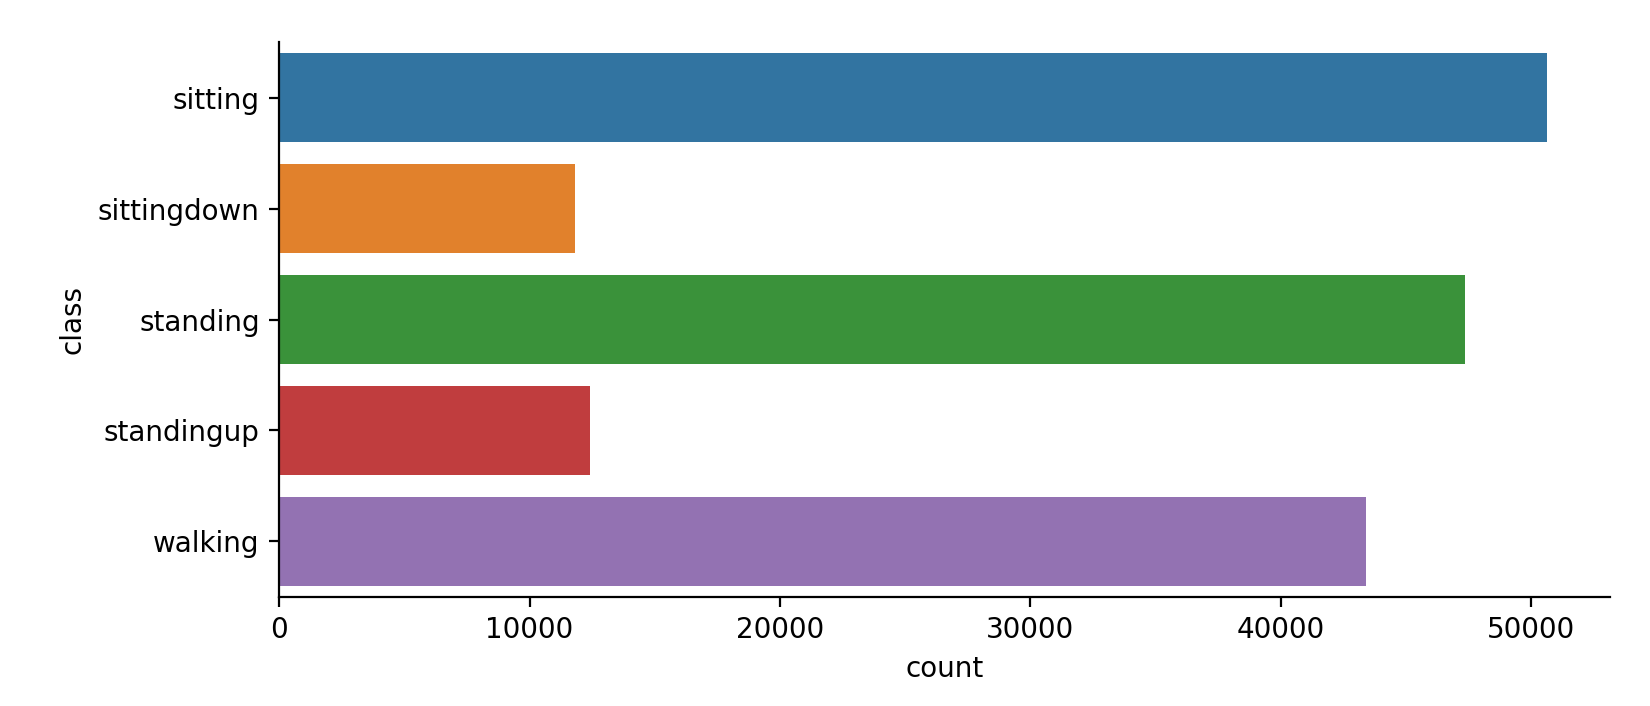
\includegraphics[width=0.8\linewidth]{bilanciamento}
    \caption{Bilanciamento della variabile target.}
    \label{fig:bilanciamento}
\end{figure}

Come si vede invece dalla figura \ref{fig:bilanciamentousers} i sample raccolti per ogni soggetto dell'esperimento sono bilanciati per tre soggetti mentre sono in misura minore per il soggetto \textit{jose\_carlos}. Dalla figura \ref{fig:classiusers} si vede invece per ogni soggetto la percentuale di sample relativi a ogni classe, e questo rispecchia il bilanciamento generale delle classi mostrato in figura \ref{fig:bilanciamento}, infatti le percentuali sono simili, in particolare le classi \textit{sittingdown} e \textit{standingup} sono presenti in misura minore.

\begin{figure}[h]
    \centering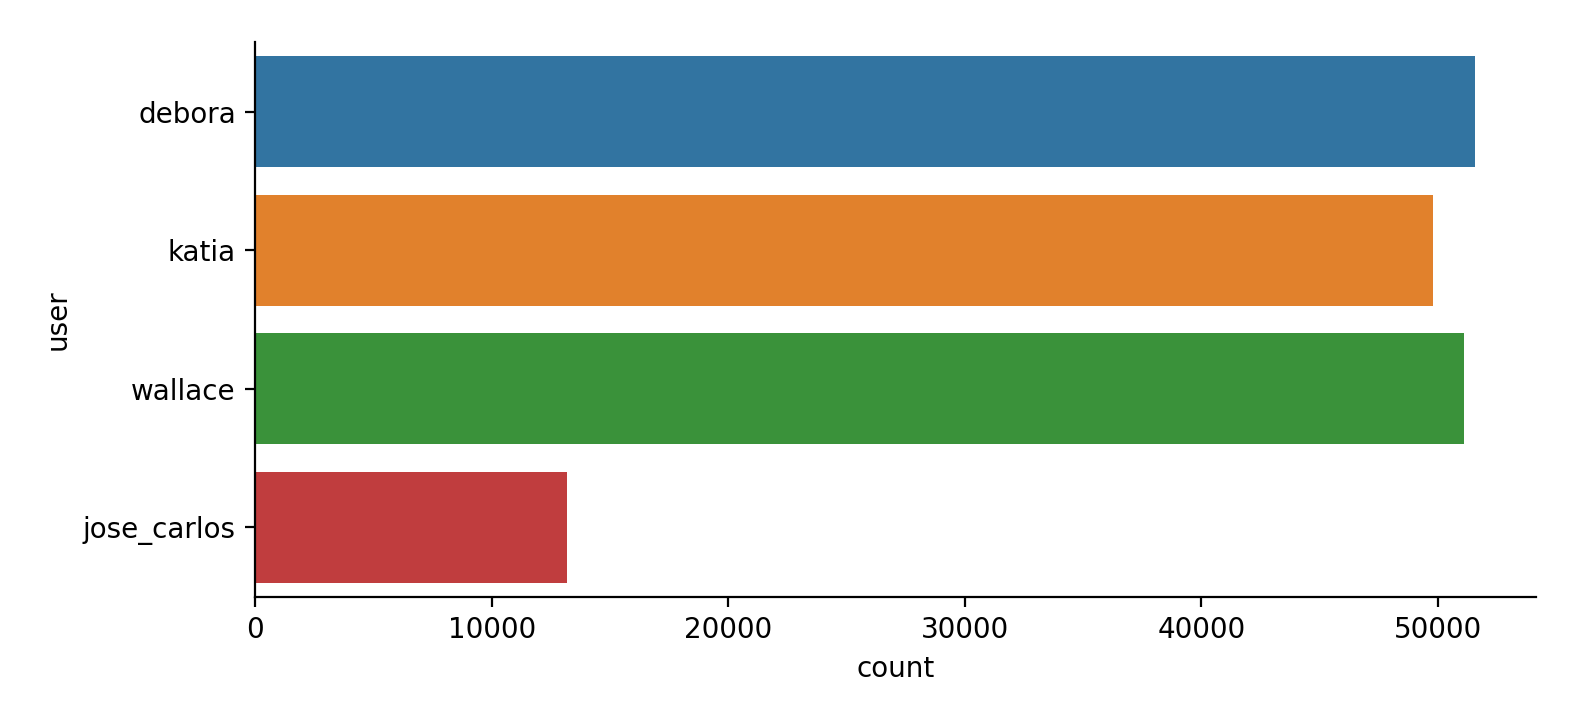
\includegraphics[width=0.5\linewidth]{bilanciamentousers}
    \caption{Bilanciamento dei dati raccolti per ogni soggetto.}
    \label{fig:bilanciamentousers}
\end{figure}

\begin{figure}[h]
    \centering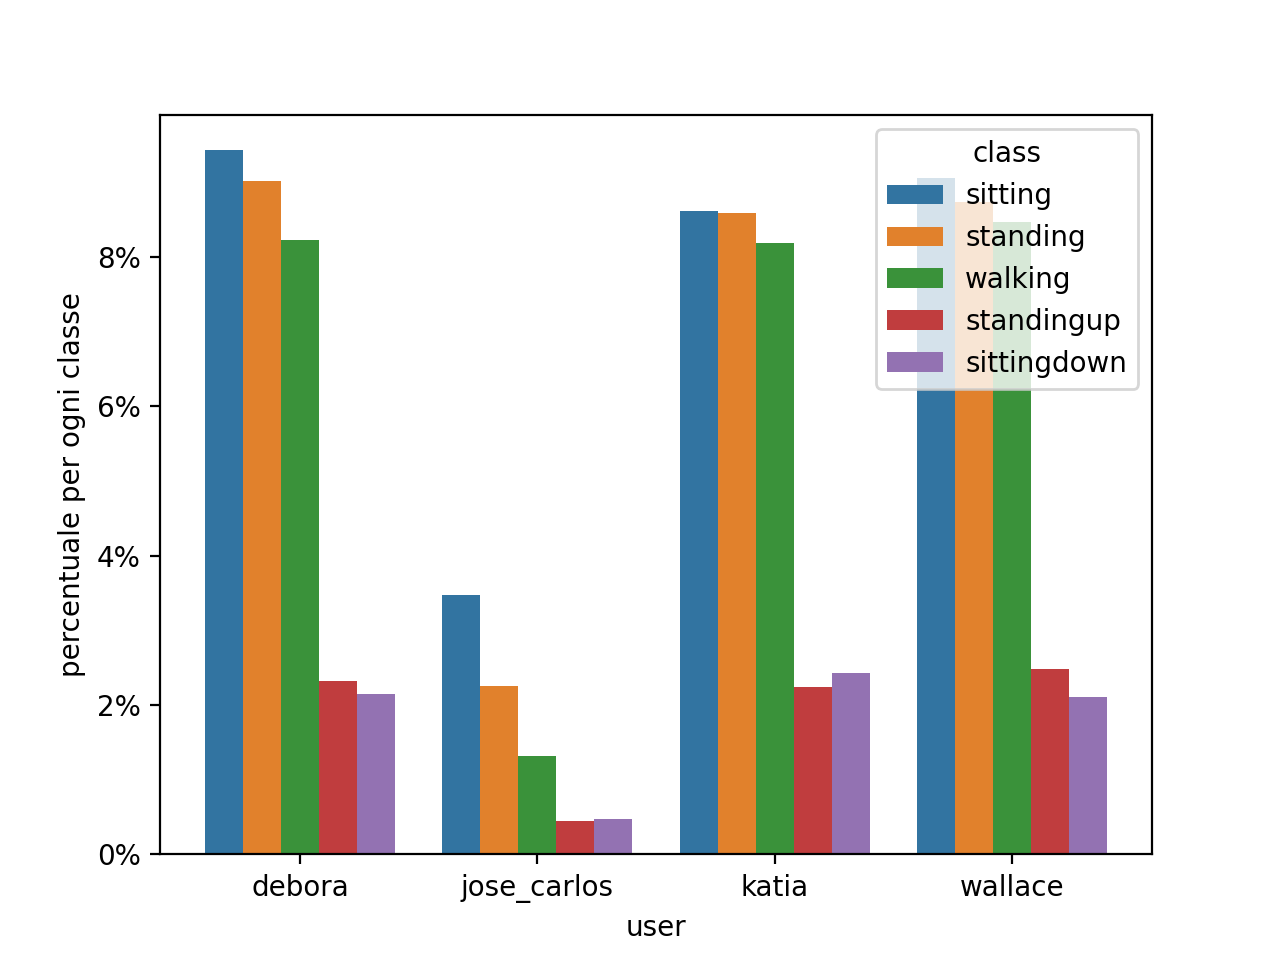
\includegraphics[width=0.5\linewidth]{divisioneclassiperuser}
    \caption{Bilanciamento delle classi per ogni soggetto.}
    \label{fig:classiusers}
\end{figure}

In figura \ref{fig:kde} sono rappresentate le distribuzioni di probabilità dei dati raccolti dall'accelerometro 2, cioè quello posto sulla coscia sinistra, classificati in base alla posizione dei soggetti. Si può notare come nel caso della classe \textit{sitting} e \textit{standing} tutte e tre le coordinate sono più concentrate nell'intorno di un unico valore, infatti la cosiddetta \textit{campana} è più stretta e alta. Questo può significare che se il valore letto è lontano dal valore di riferimento difficilmente la posizione sarà una delle due tra \textit{sitting} e \textit{standing}.

\begin{figure}[h]
    \centering
    \begin{subfigure}[t]{0.4\textwidth}
        \centering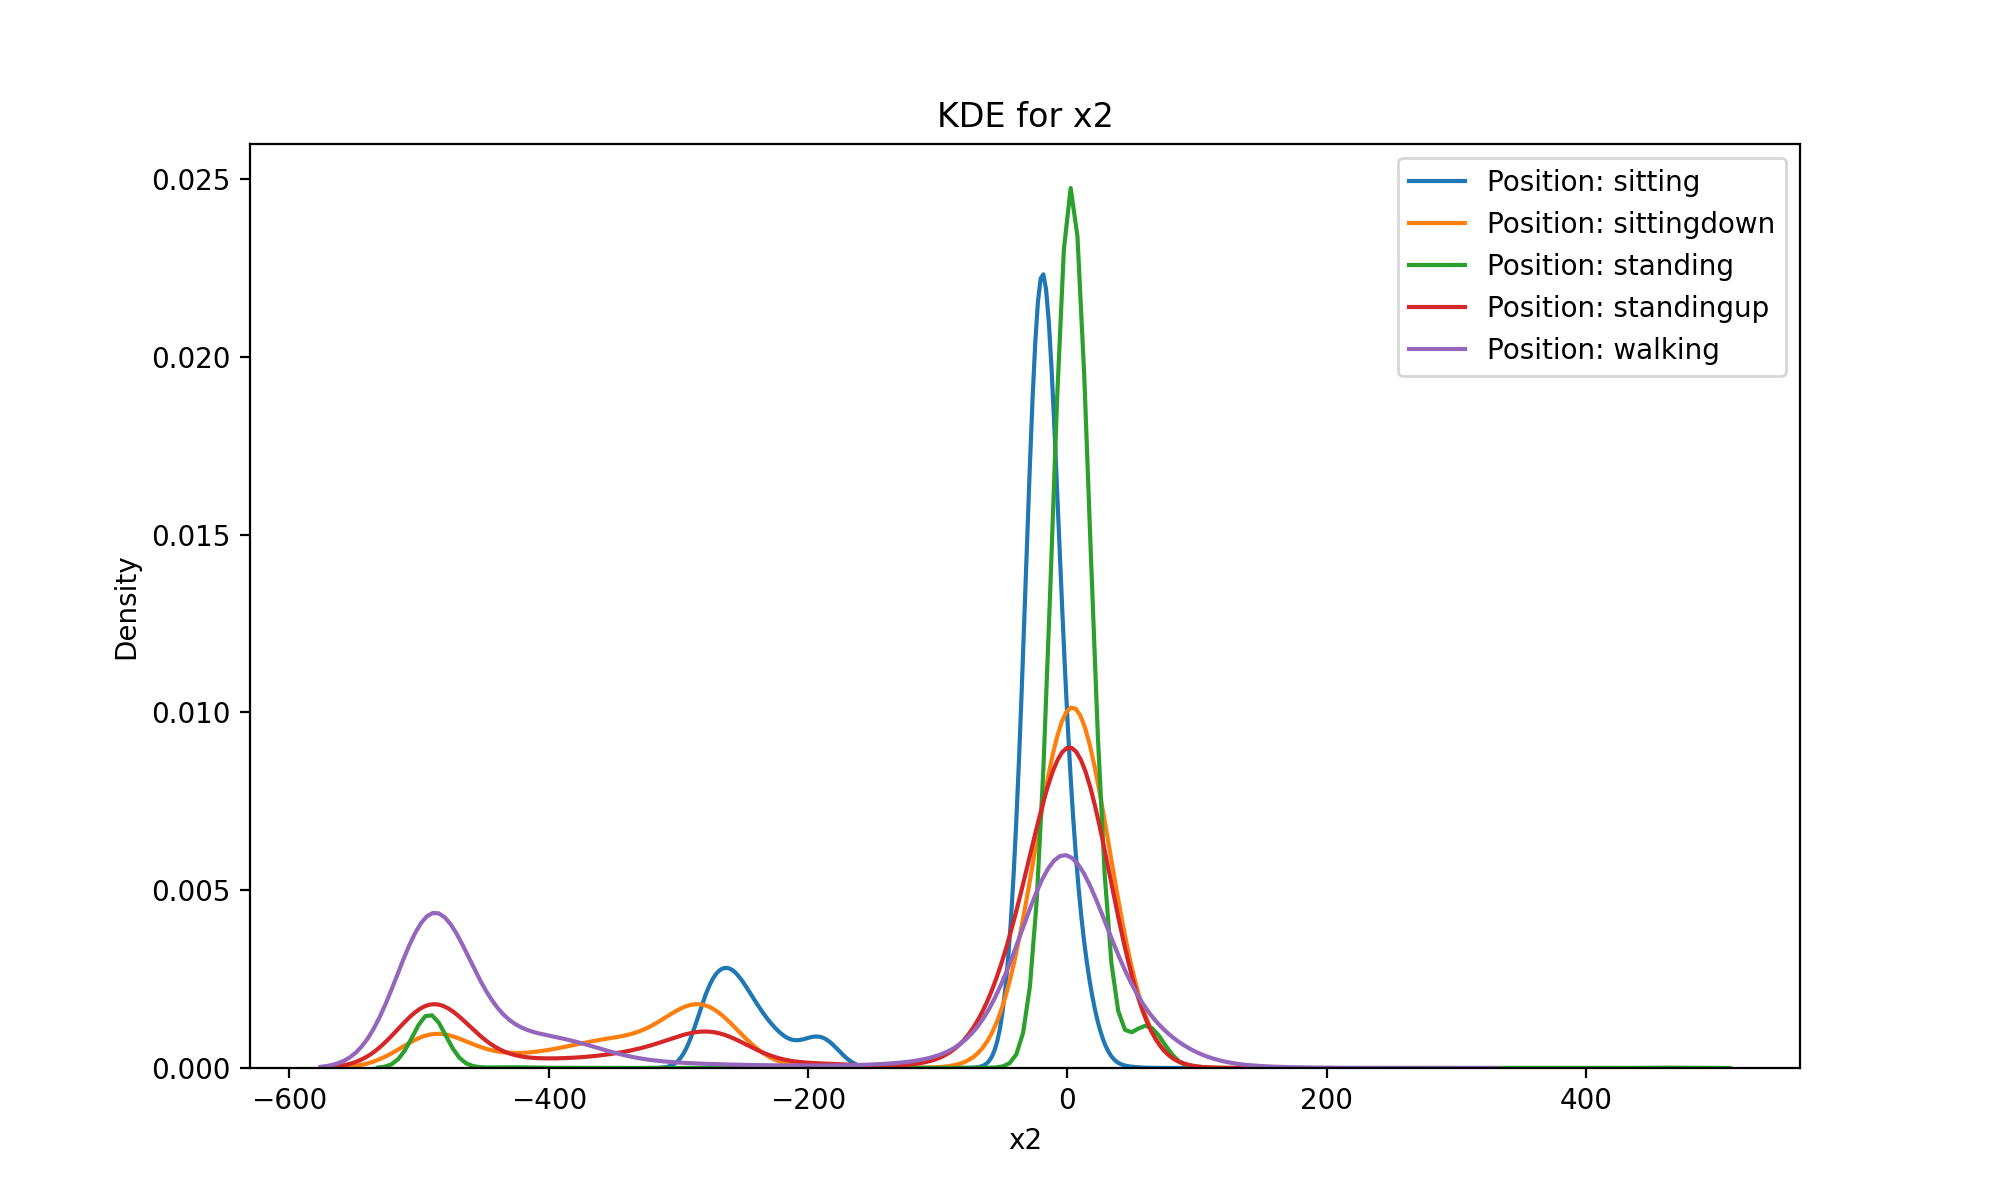
\includegraphics[width=1\linewidth]{x2}
        \caption{Distribuzione della coordinata x.}
        \label{fig:kde:x2}
    \end{subfigure}
    %
    \begin{subfigure}[t]{0.4\textwidth}
        \centering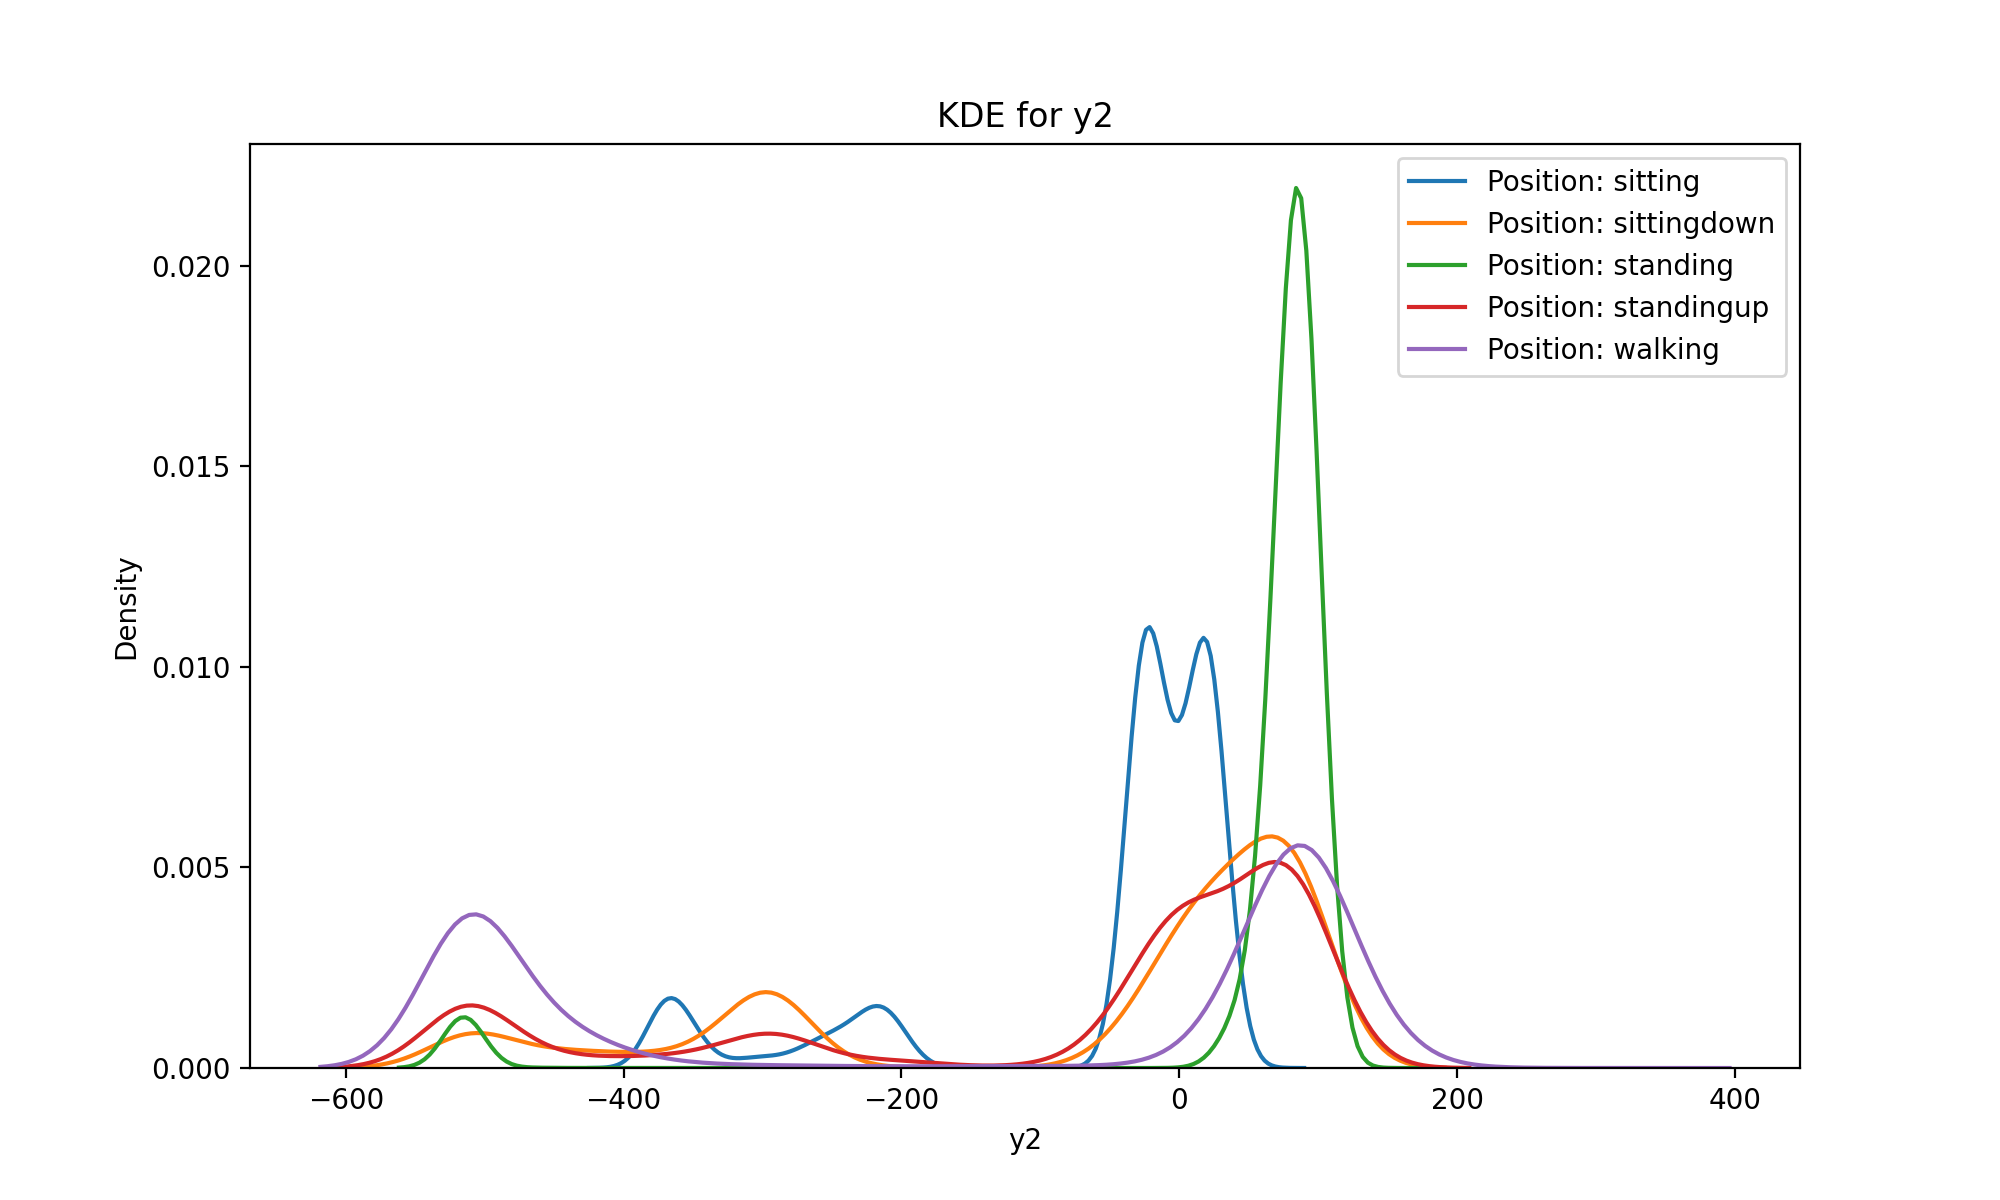
\includegraphics[width=1\linewidth]{y2}
        \caption{Distribuzione della coordinata y.}
        \label{fig:kde:y2}
    \end{subfigure}
    %
    \\
    \begin{subfigure}[t]{0.4\textwidth}
        \centering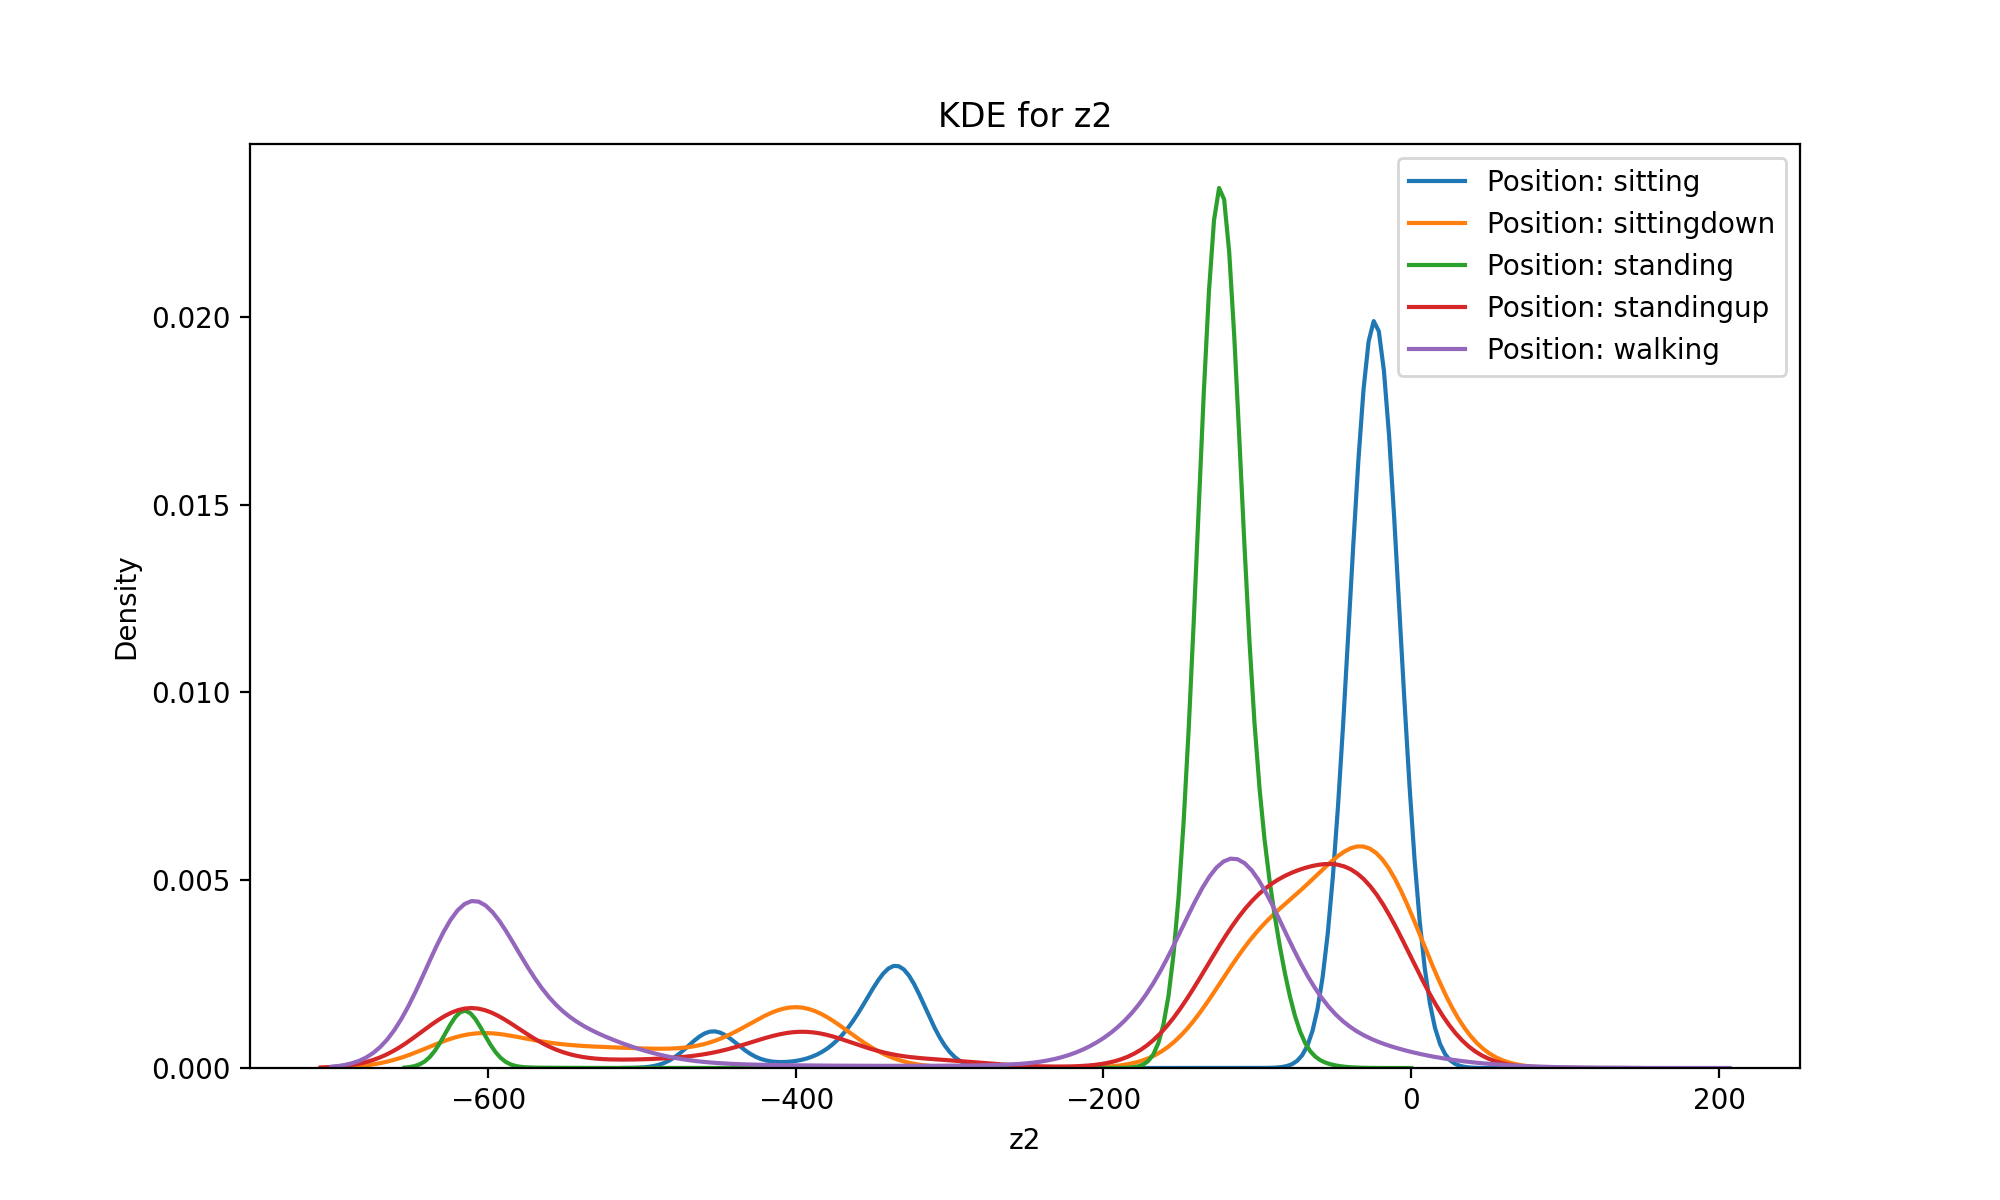
\includegraphics[width=1\linewidth]{z2}
        \caption{Distribuzione della coordinata z.}
        \label{fig:kde:z2}
    \end{subfigure}
    %
    \caption{Densità delle coordinate dell'accelerometro 2.}
    \label{fig:kde}
\end{figure}

Nella figura \ref{fig:pairplot} si vede la relazione tra le coordinate dell'accelerometro 2 e le coordinate di tutti gli accelerometri divisi per classe. Le informazioni utili che si ricavano da questo grafico sono che le coordinate dell'accelerometro 3, quello sulla caviglia destra, differiscono da quelle dell'accelerometro 2 nel caso di posizione \textit{standingup} e \textit{walking}, infatti la zona rossa, che rappresenta la posizione \textit{standingup}, assume valori minori in termini di coordinate dell'accelerometro 3. Il resto delle classi non sono distinguibili e le coordinate assumono un range di valori simile tra loro.

\begin{figure}[h]
    \centering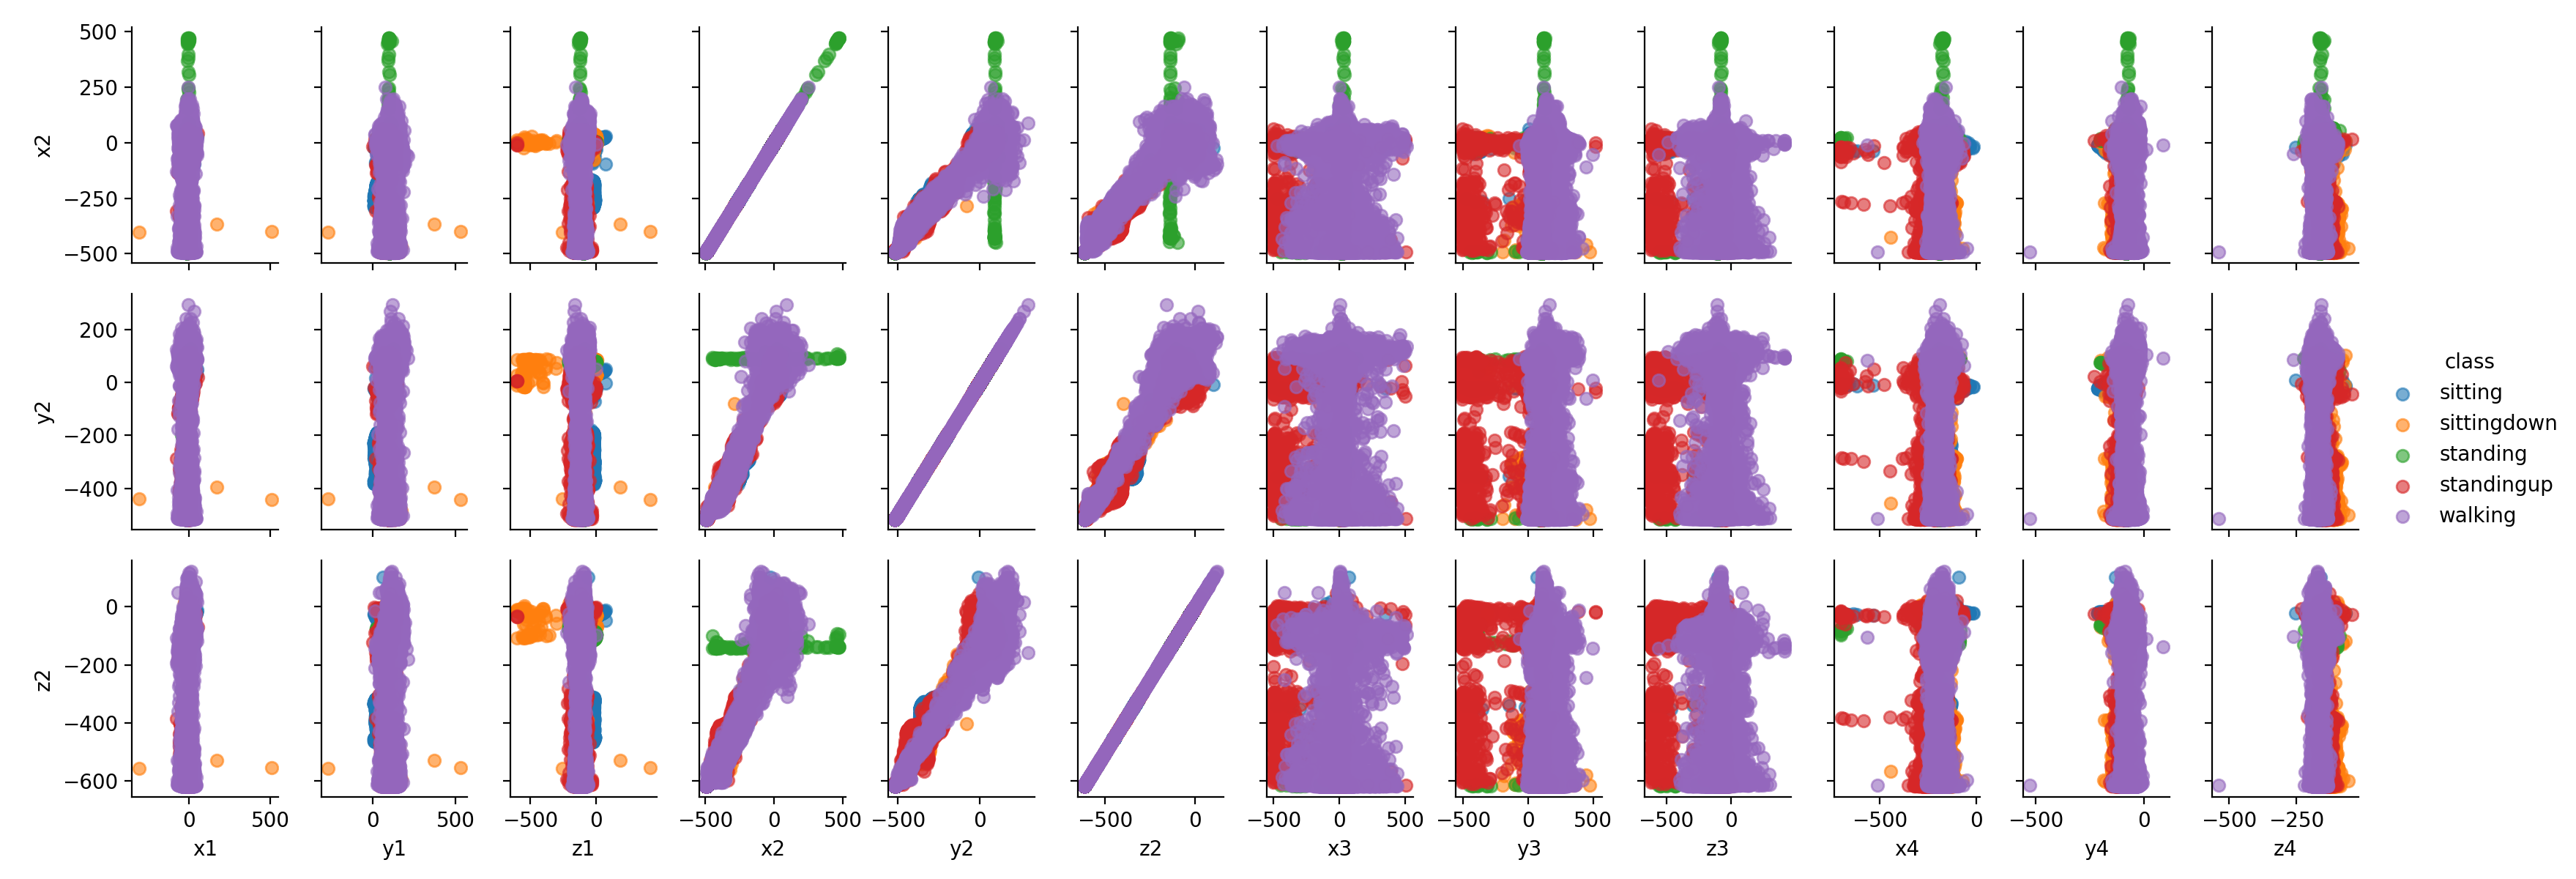
\includegraphics[width=1.0\linewidth]{pairplotacc2}
    \caption{Pairplot delle coordinate dell'accelerometro 2.}
    \label{fig:pairplot}
\end{figure}

L'accelerometro 1, quello posto sulla vita, legge delle coordinate a seconda della posizione che sono rappresentate in figura \ref{fig:scatterplot}. Come si vede dai tre grafici rappresentanti le tre coordinate, i valori non variano molto al variare della posizione, eccezion fatta per la coordinata z che diminuisce il suo valore in posizione \textit{sitting down}. Questa informazione è ragionevole, infatti la vita è la parte del corpo che cambia meno la sua posizione nello spazio al variare della postura.  Quando ci siede invece l'altezza della vita (rappresentata dalla coordinata z) si abbassa e quindi diminuisce la coordinata relativa. Inoltre dai grafici \ref{fig:scatterplot:x1}, \ref{fig:scatterplot:y1}, \ref{fig:scatterplot:z1} è possibile notare degli high leverage point presenti nei dati, cioè quei sample che differiscono dagli altri in termini di valore di una feature, in questo caso le feature \textit{x1}, \textit{y1} e \textit{z1}.

\begin{figure}[h]
    \centering
    \begin{subfigure}[t]{0.4\textwidth}
        \centering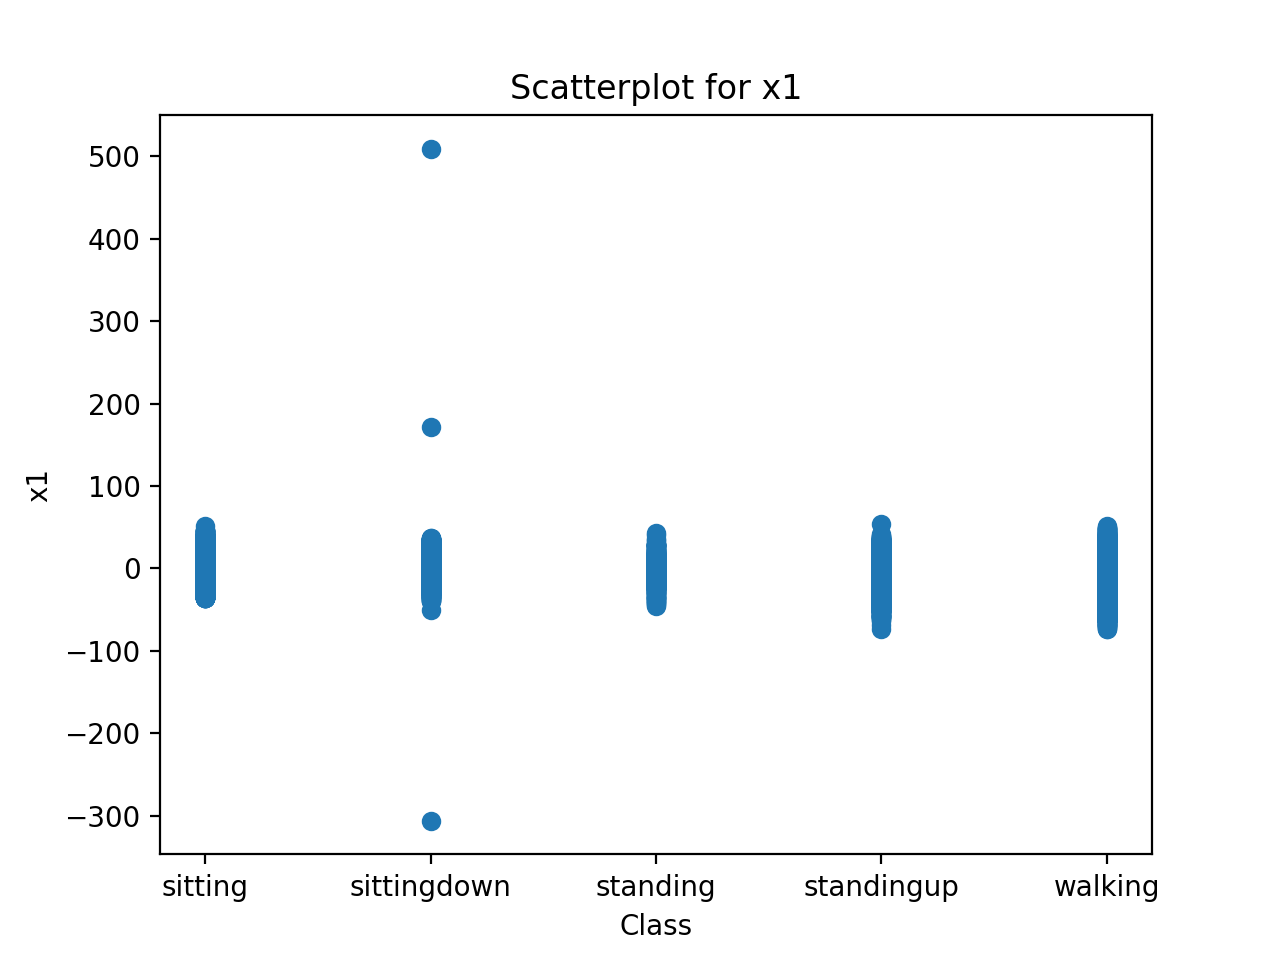
\includegraphics[width=1\linewidth]{scatx1}
        \caption{Scatterplot della coordinata x.}
        \label{fig:scatterplot:x1}
    \end{subfigure}
    %
    \begin{subfigure}[t]{0.4\textwidth}
        \centering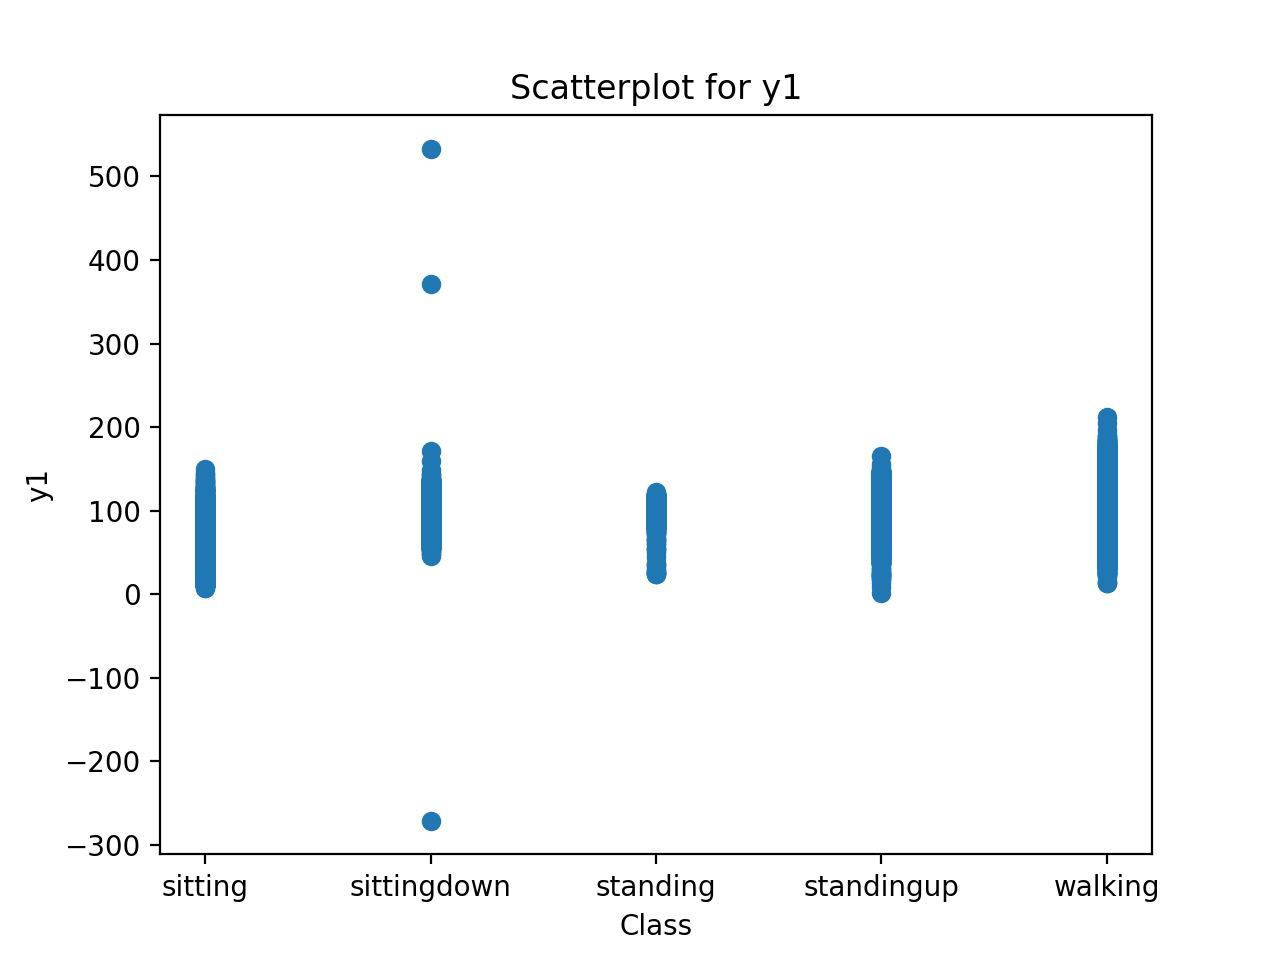
\includegraphics[width=1\linewidth]{scaty1}
        \caption{Scatterplot della coordinata y.}
        \label{fig:scatterplot:y1}
    \end{subfigure}
    %
    \\
    \begin{subfigure}[t]{0.4\textwidth}
        \centering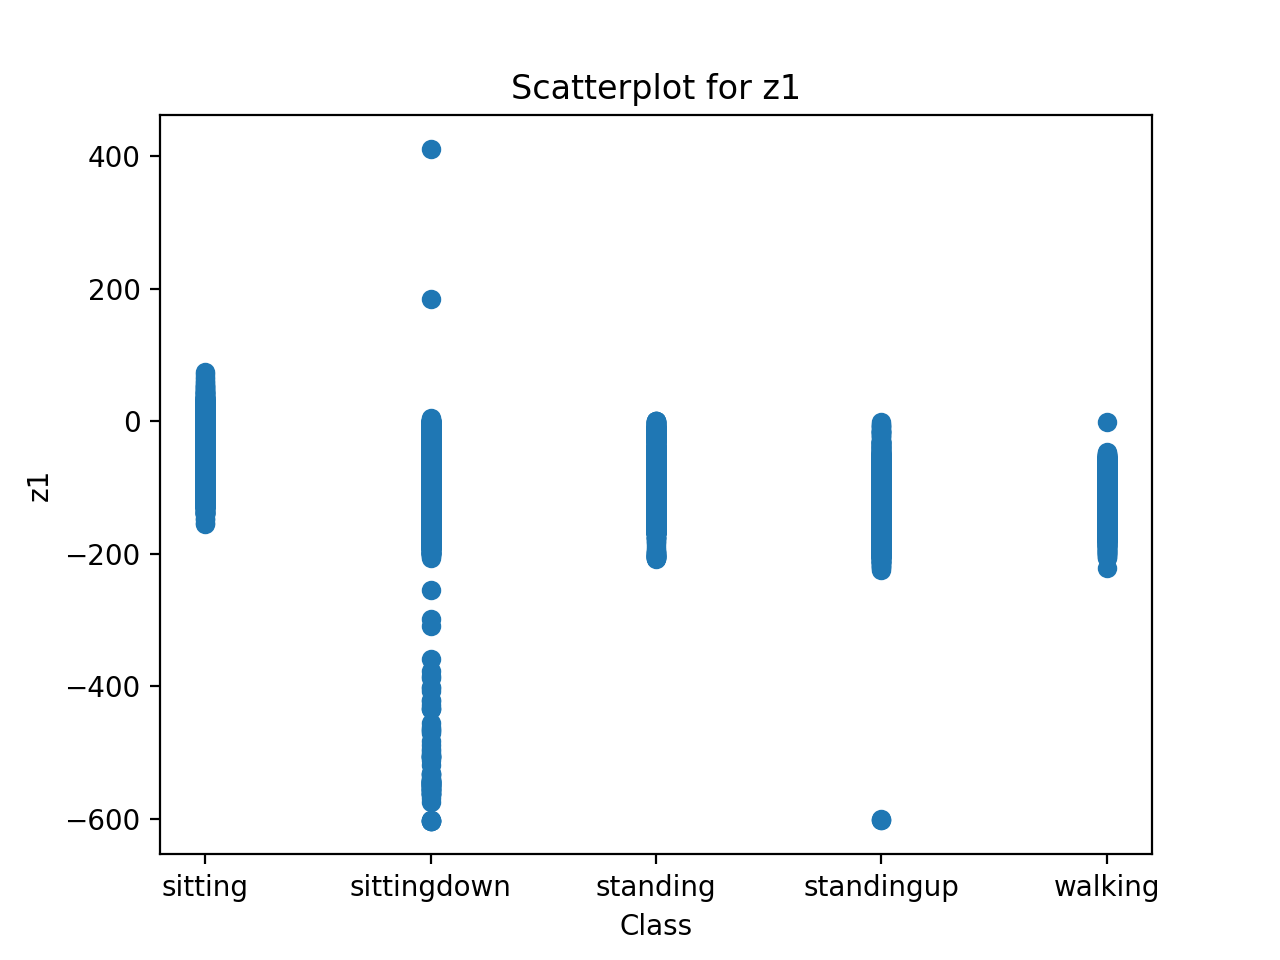
\includegraphics[width=1\linewidth]{scatz1}
        \caption{Scatterplot della coordinata z.}
        \label{fig:scatterplot:z1}
    \end{subfigure}
    %
    \caption{Scatterplot delle coordinate dell'accelerometro 1.}
    \label{fig:scatterplot}
\end{figure}

Nella fase di pre-processing delle variabili è stato fatto un encoding delle features categoriche, in particolare la feature \textit{gender} è stata trasformata con un oggetto di tipo \verb+LabelEncoder()+, che ha mappato i due possibili valori, \textit{man} e \textit{woman}, in numeri, \textit{0} e \textit{1} rispettivamente.  Inoltre è stato fatto l'encoding con lo stesso metodo anche della variabile target, \textit{class}, mappando le cinque classi con numeri da \textit{0} a \textit{4}. Dopodiché è stato effettuato il min-max-scaling alle features, che porta il valore di ogni feature tra 0 e 1, per velocizzare il training dei modelli.  Inoltre per alcuni modelli è stato deciso di fare una riduzione delle features tramite la PCA (Principal Component Analysis), che sarà però approfondita nella sezione \ref{sec:implementazione}.
Infine il criterio di splitting scelto per il dataset è stato il seguente:
\begin{itemize}
\item \textbf{training set}: 80\% del dataset originale
\item \textbf{test set}: 20\% del dataset originale
\end{itemize}
Lo splitting è stato fatto in modo stratificato in modo da effettuare la divisione mantenendo bilanciate le classi della variabile target.

In fase di cross validazione sarà poi effettuato un ulteriore splitting del training set, in validation set e development set per fare la model selection per la scelta opportuna dei parametri dei vari modelli, e la model assessment per stimare le prestazioni dei modelli. 
\section{Discussione dei modelli}\label{sec:modelli}
Il problema in esame è un problema di classificazione perché è necessario appunto "classificare" la postura di un soggetto tra cinque possibili posizioni. Gli algoritmi di machine learning adatti a questo tipo di problema sono diversi, i principali sono la \textit{softmax regression},  è come la logisitc regression ma per il caso multiclasse e utilizza la funzione softmax invece della funzione logisitica; il \textit{classificatore naive Bayes}, basato principalmente sul teorema della probabilità di Bayes; il \textit{K-Nearest neighbors}, che assume che sample simili siano vicini nello spazio delle features, quindi calcola la distanza relativa tra le features e per ogni sample prende i K samples più vicini e ne restituisce la moda delle label. Il parametro K è quindi un iperparametro da scegliere opportunamente. Il \textbf{decision tree}, o \textbf{alber decisionale} in italiano, è un metodo di apprendimento nel quale i dati sono suddivisi in base a un certo parametro in sottoinsiemi sempre più piccoli, fino ad arrivare ad avere insiemi che non sono più divisibili, questi saranno le foglie dell'albero e definiranno la label. In particolare gli alberi decisionali sono composti da:
\begin{itemize}
\item \textbf{nodi}: controllano il valore di un determinato parametro sui dati,
\item \textbf{rami}: collegano più nodi e rappresentano l'esito di un test fatto dal nodo padre,
\item \textbf{foglie}: sono i nodi terminali e determinano il risultato finale.
\end{itemize}

Per selezionare le features su cui effettuare il test e il valore \textit{cutpoint}, cioè il valore limite da testare, si utilizza il \textbf{recursive binary splitting} che ad ogni passo seleziona le features e il cutpoint che riducono maggiormente l'impurità dei nodi, un nodo è puro quando tutti i samples appartenenti alla medesima suddivisione hanno la stessa label.  L'indice per misurare l'impurità è un iperparametro e può essere scelto, una possibile soluzione è usare l'indice di Gini, cioè la probabilità che un una variabile sia classificata in modo errato. Uno dei vantaggi degli alberi decisionali è che sono semplici da costruire e veloci, inoltre escludono in modo automatico le features non importanti, ha però lo svantaggio di tendere facilmente all'overfitting. 

Un altro modello adatto a questo problema è il \textbf{support vector machine} (SVM), infatti il SVM ha lo scopo di dividere i sample in classi con un iperpiano di uno spazio n-dimensionale, dove n è il numero delle features. L'iperpiano da scegliere è quello con il massimo margine, cioè la massima distanza tra sample di classi diverse. Un aspetto fondamentale del SVM è che se i sample non fossero divisibili in modo lineare è possibile applicare una trasfomazione non lineare ai dati, per portarli in uno spazio con più dimensioni nel quale sono divisibili in modo lineare, la funzione che effettua questa trasformazione non lineare è detta \textbf{kernel} e può essere scelta in base al problema specifico, possibili scelte sono il kernel polinomiale o la radial basis function (RBF). Inoltre non sempre i sample sono divisibili perfettamente ma è necessario commettere degli errori, in questo caso si utilizza il \textbf{coefficiente di regolarizzazione} (C), un iperparametro per gestire il bilanciamento tra errori commessi e la grandezza del margine: per C piccolo si dà più importanza al margine, mentre per C grande si cerca di evitare più errori possibile. L'SVM ha il vantaggio di occupare poca memoria ed essere molto efficace in caso di dimensionalità delle features molto elevata, grazie all'utilizzo dei kernel.

L'ultimo metodo di learning approfondito sono le \textbf{reti neurali}. Una rete è composta da diversi \textit{layer}, e ogni layer ha diversi \textit{nodi}. Le features sono messe in input al primo layer, che a sua volta calcolerà una combinazione lineare degli ingressi e poi ne farà una trasformazione non lineare secondo una certa \textit{funzione di attivazione}, dopodiché l'output del primo layer è mandato in input al secondo layer. Questo processo è iterato fino ad arrivare all'ultimo layer, che calcolerà l'output finale. Il numero di layer e il numero di nodi per ogni layer è un iperparametro da scegliere opportunamente, inoltre è possibile scegliere la funzione di attivazione da applicare ai dati, in particolare le funzioni cosiddette "S-shaped", come la funzione sigmoide e la funzione tangente iperbolica (tanh) caratterizzano le reti chiamate \textit{multilayer perceptron} (MLP).  Un'altra componente fondamentale delle reti neurali sono i pesi che ogni collegamento tra nodi di livelli diversi ha, questi pesi sono i valori che il modello deve imparare durante la fase di training, per farlo le reti neurali usano il \textbf{error backporpagation}: si confronta il valore in uscita con il valore reale atteso, e in base all'errore, cioè alla differenza tra i due, si modificano i pesi. Un alto numero di layer e di nodi può portare a overfitting e ad alta complessità, per evitare questo problema di utilizzano delle tecniche di regolarizzazione, come il \textbf{weight decay} e l'\textbf{early stopping}. Un difetto delle reti neurali è la loro lentezza nel training dovuta proprio all'applicazione dell'algoritmo di error backpropagation, infatti le reti neurali richiedono molte risorse computazionali e l'addestramento risulta quindi lento.

Per questo progetto è stato scelto di utilizzare tre dei modelli descritti:
\begin{itemize}
\item Decision Tree,
\item Support Vector Machine
\item Reti Neurali
\end{itemize}

In particolare per ogni modello saranno studiate tre versioni:
\begin{itemize}
\item versione 1: i modelli sono addestrati con i dati grezzi e originali, senza pre-processing,
\item versione 2: i modelli sono addestrati con i dati pre-processati,
\item versione 3: si utilizza una versione ensemble della versione migliore tra le prime due
\end{itemize}
\section{Dettagli implementativi}\label{sec:implementazione}
In questo paragrafo verranno descritti in modo specifico i dettagli implementativi di ogni modello e di ogni sua versione, oltre ai vari passaggi di pre-processing e il metodo di valutazione.

\subsection{Pre-processing}
Per le versioni 1 dei modelli i dati non vengono pre-processati, infatti i dati non vengono pre-processati come descritto nella sezione \ref{sec:analisi}, ma vengono solamente fatte le modifiche in fase di EDA, modificando quindi i tipi dei dati ed eliminando i valori NaN. Lo splitting in questo caso è fatto quindi sui dati originali, togliendo dalle features lo \textit{user}, che è il nome del soggetto e non influisce sull'apprendimento, ed è stato tolta anche la feature \textit{gender}, in quanto non ancora trasformata con l'encoder. Inoltre la variabile target \textit{class} in questo caso rimane sottoforma di stringa.

Per le versioni 2 invece vengono effettuati gli step di pre-processing descritti brevemente nella sezione \ref{sec:analisi}, in particolare dopo aver fatto l'encoding della feature \textit{gender} e del target \textit{class}, è stata studiata la matrice di correlazione, mostrata in figura \ref{fig:corr}, per valutare la collinearità tra features tra di loro, e con la variabile target. Ne risulta che le variabili \textit{y1} e \textit{y4} sono particolarmente correlate con la variabile target, quindi saranno importanti ai fini della classificazione. In secondo luogo è possibile notare che le features \textit{how\_tall\_in\_meters}, \textit{weight} e \textit{body\_mass\_index} sono particolarmente correlate tra di loro e di conseguenza è conveniente eliminarne due mantenerne una sola. Infine le tre variabili che rappresentano le coordinate dell'accelerometro 2, quello sulla coscia sinistra, sono molto correlate tra loro, quindi anche in questo caso conviene mantenerne una sola.

\begin{figure}[ht]
    \centering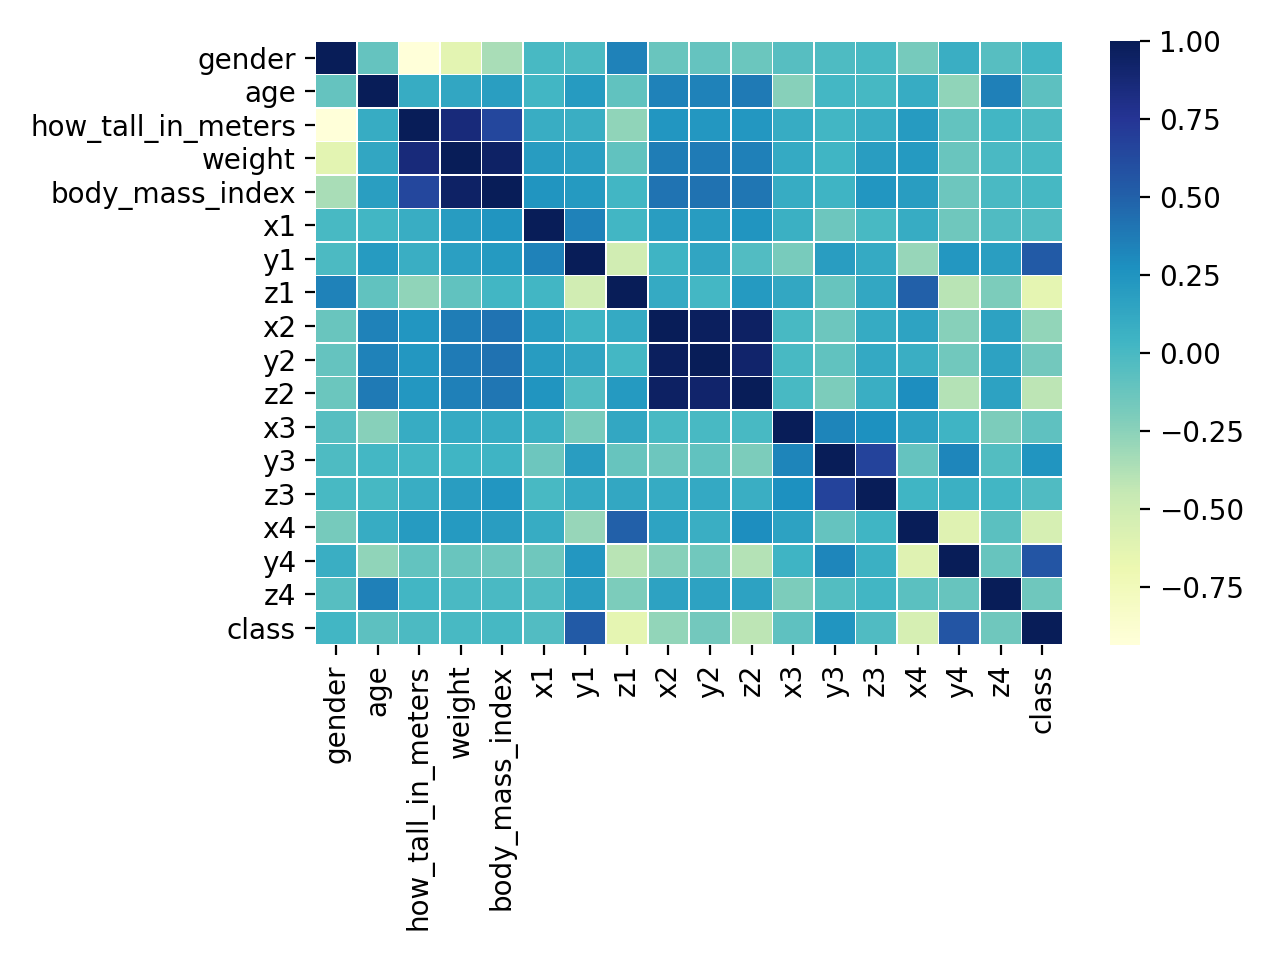
\includegraphics[width=1.0\linewidth]{corr}
    \caption{Matrice di correlazione.}
    \label{fig:corr}
\end{figure}

Dalle informazioni raccolte dalla matrice di correlazione, in figura \ref{fig:corr}, effettuiamo la features selection eliminando le variabili \textit{weight} e \textit{body\_mass\_index} perchè altamente correlate con \textit{how\_tall\_in\_meters} e viene mantenuta quest'ultima; vengono anche eliminate le coordinate x e z del secondo accelerometro, mantenendo solo la coordinata y. Infine vengono eliminate le variabili \textit{user} e \textit{age} in quanto non influenti sul riconoscimento della postura.

Le features selezionate vengono poi sottoposte a uno scaling, in particolare di applica il metodo del \textbf{min-max-scaling}: trasforma il valore di ogni features portandolo a un valore compreso tra 0 e 1, per farlo applica a ogni variabile la seguente formula:

\begin{equation}
x' = \frac{x-min(x)}{max(x)-min(x)}
\end{equation}

È importante sottolineare che i parametri $min(x)$ e $max(x)$ vanno calcolati sulla base del solo training set, dopodiché si applica la trasformazione al training set e al test set.

\begin{figure}[ht]
    \centering
    \begin{subfigure}[t]{0.4\textwidth}
        \centering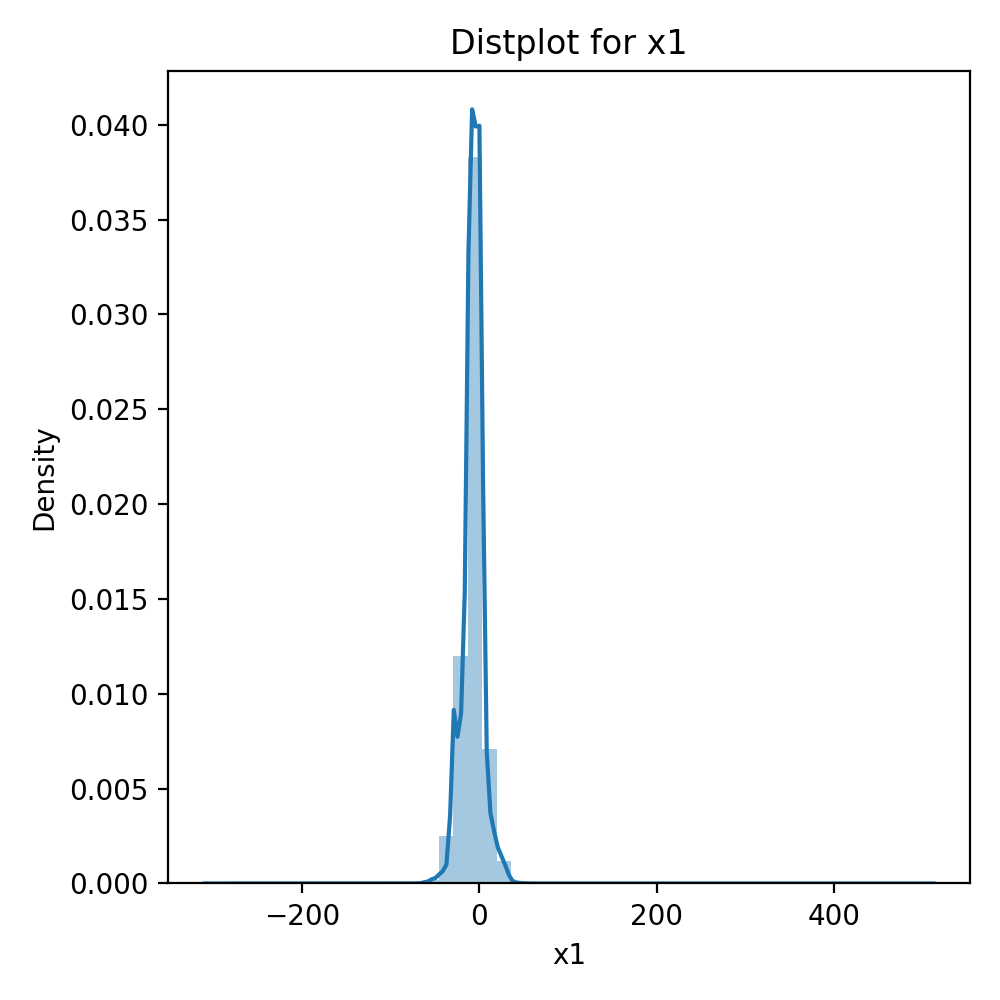
\includegraphics[width=1\linewidth]{x1prescaling}
        \caption{Distribuzione di x1 prima del min-max-scaling.}
        \label{fig:distprescaling:x1}
    \end{subfigure}
    %
    \begin{subfigure}[t]{0.4\textwidth}
        \centering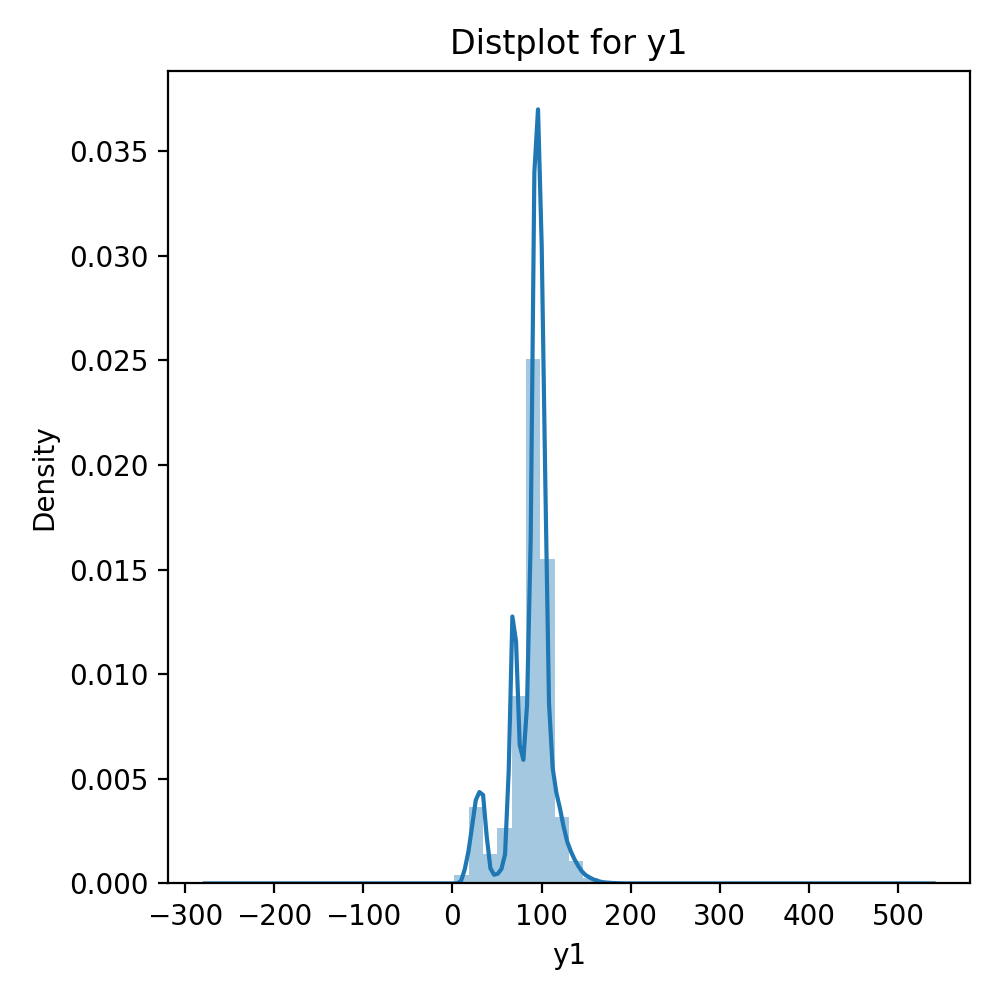
\includegraphics[width=1\linewidth]{y1prescaling}
        \caption{Distribuzione di y1 prima del min-max-scaling.}
        \label{fig:distprescaling:y1}
    \end{subfigure}
    %
    \\
    \begin{subfigure}[t]{0.4\textwidth}
        \centering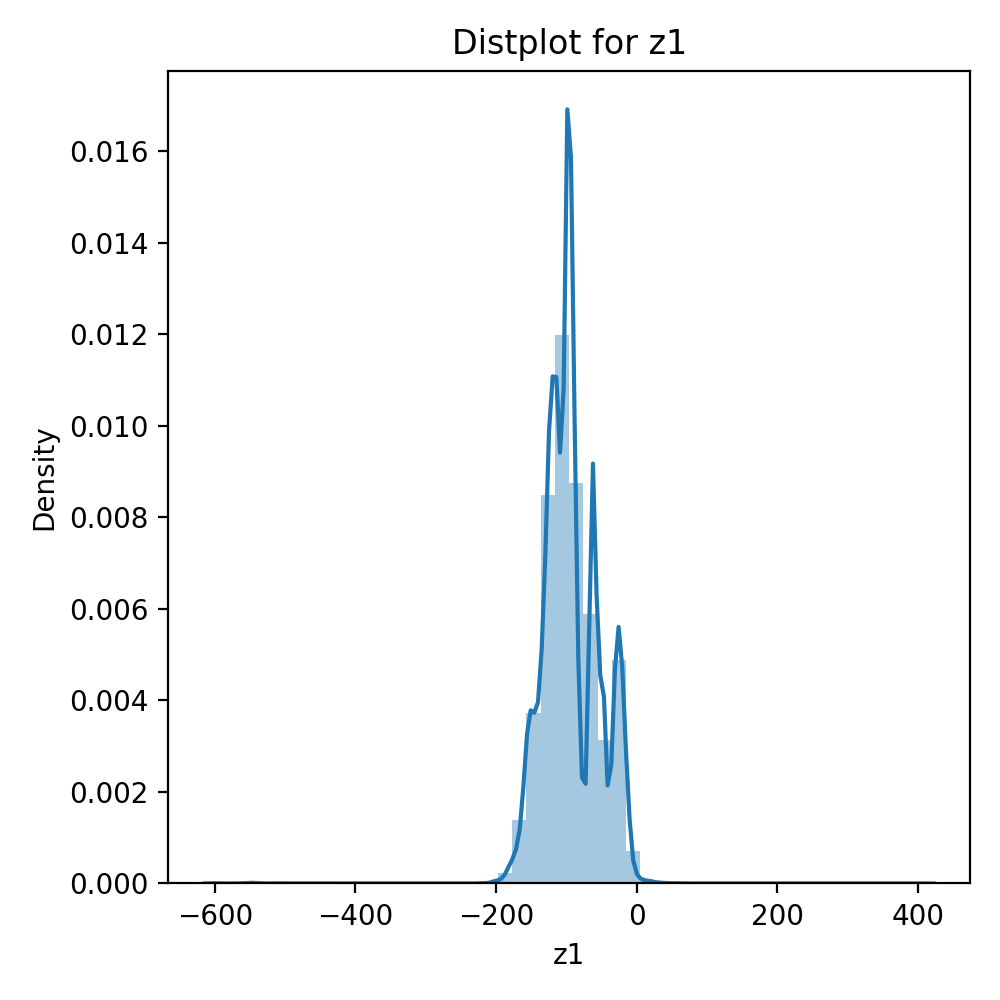
\includegraphics[width=1\linewidth]{z1prescaling}
        \caption{Distribuzione di z1 prima del min-max-scaling.}
        \label{fig:distprescaling:z1}
    \end{subfigure}
    %
    \begin{subfigure}[t]{0.4\textwidth}
        \centering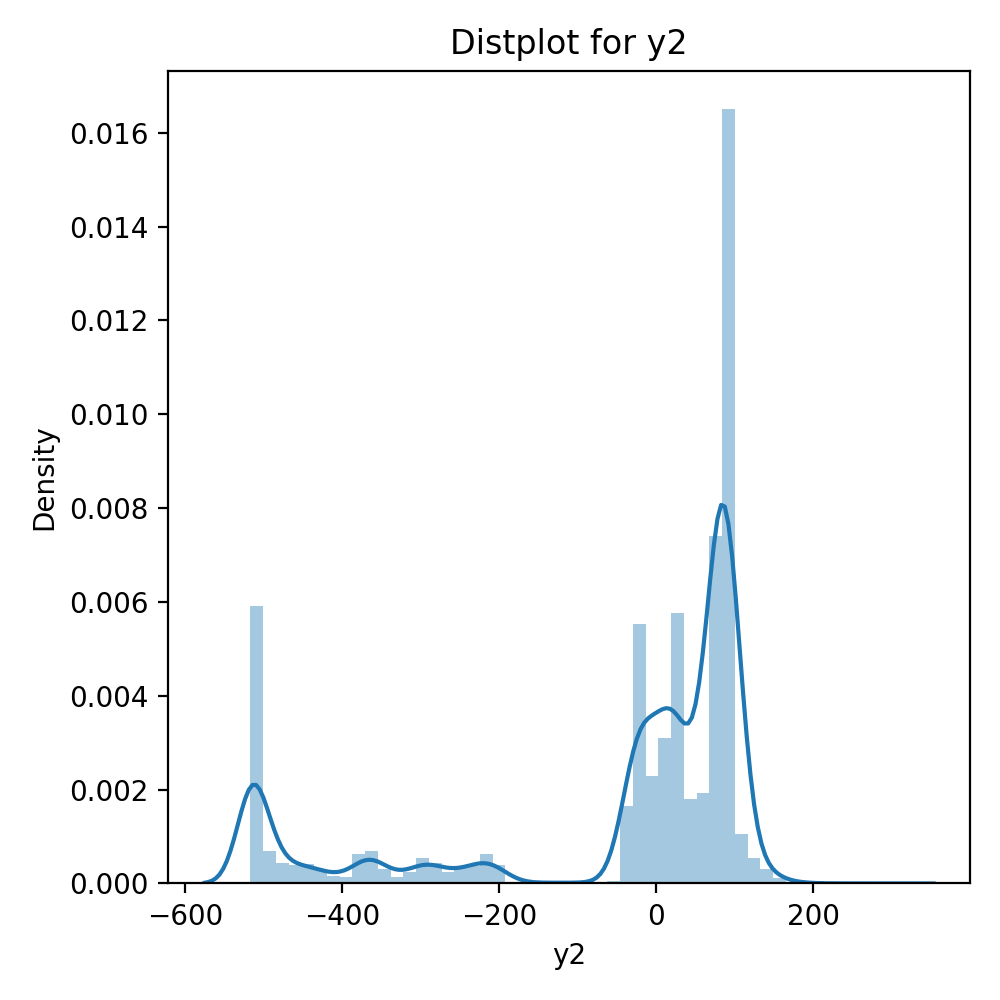
\includegraphics[width=1\linewidth]{y2prescaling}
        \caption{Distribuzione di y2 prima del min-max-scaling.}
        \label{fig:distprescaling:y2}
    \end{subfigure}
    \caption{Distribuzione di variabili prima del min-max-scaling.}
    \label{fig:distprescaling}
\end{figure}

In figura \ref{fig:distprescaling} sono mostrati i grafici di distribuzione di alcune variabili prima di aver subito il min-max-scaling, come si vede i valori variano nell'ordine delle centinaia intorno allo zero.

\begin{figure}[ht]
    \centering
    \begin{subfigure}[t]{0.4\textwidth}
        \centering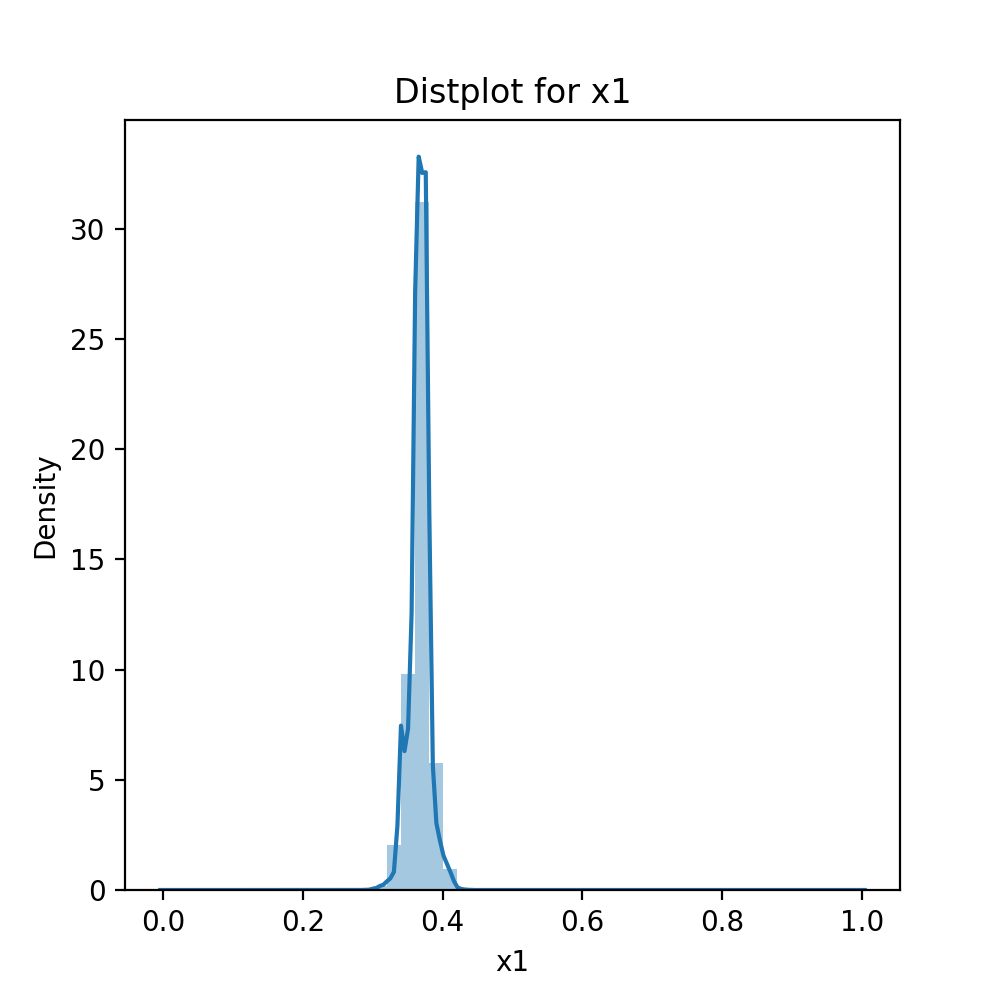
\includegraphics[width=1\linewidth]{x1postscaling}
        \caption{Distribuzione di x1 dopo il min-max-scaling.}
        \label{fig:distpostscaling:x1}
    \end{subfigure}
    %
    \begin{subfigure}[t]{0.4\textwidth}
        \centering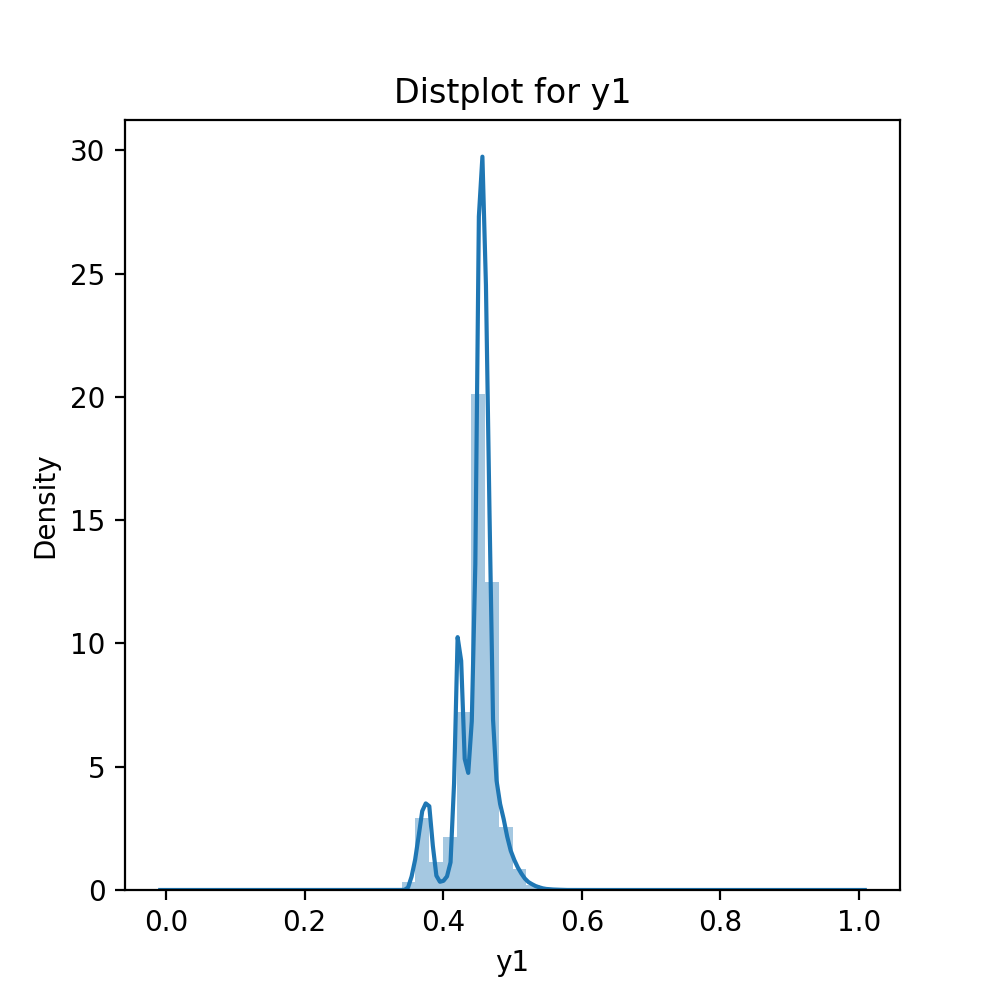
\includegraphics[width=1\linewidth]{y1postscaling}
        \caption{Distribuzione di y1 dopo il min-max-scaling.}
        \label{fig:distpostscaling:y1}
    \end{subfigure}
    %
    \\
    \begin{subfigure}[t]{0.4\textwidth}
        \centering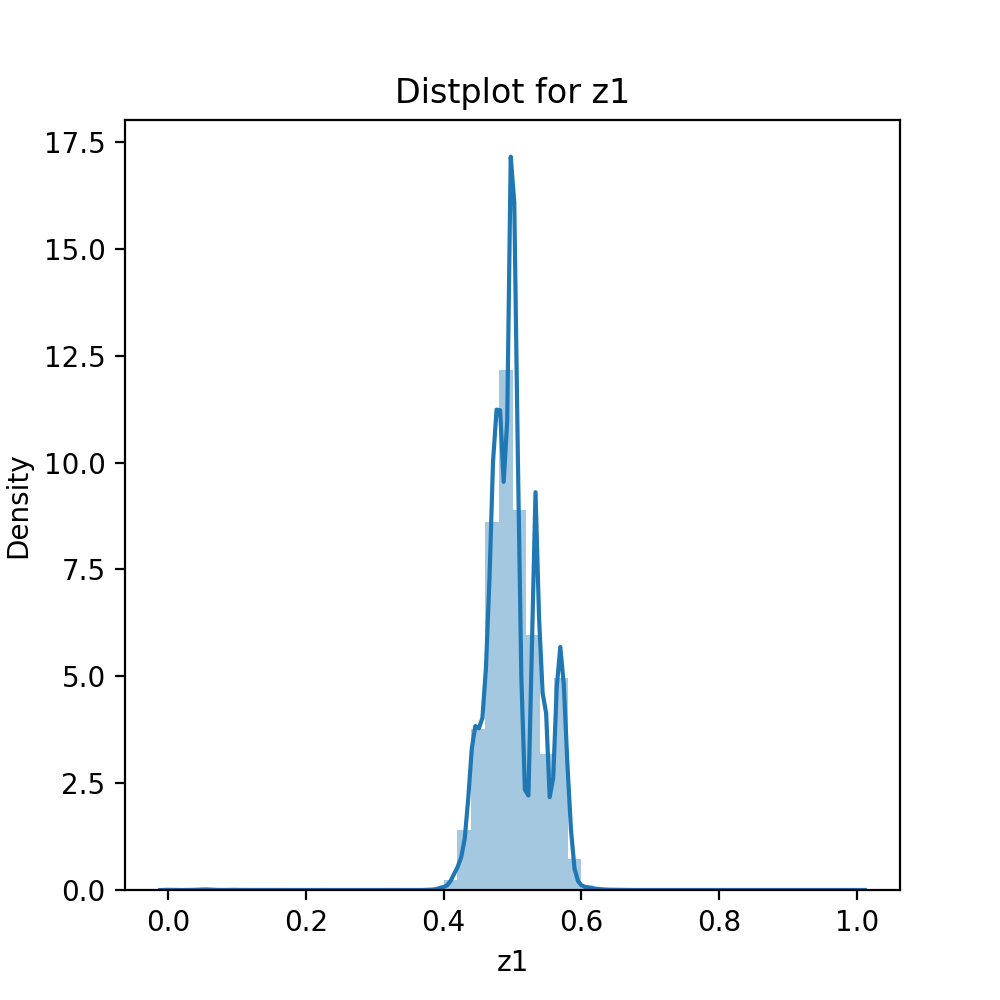
\includegraphics[width=1\linewidth]{z1postscaling}
        \caption{Distribuzione di z1 dopo il min-max-scaling.}
        \label{fig:distpostscaling:z1}
    \end{subfigure}
    %
    \begin{subfigure}[t]{0.4\textwidth}
        \centering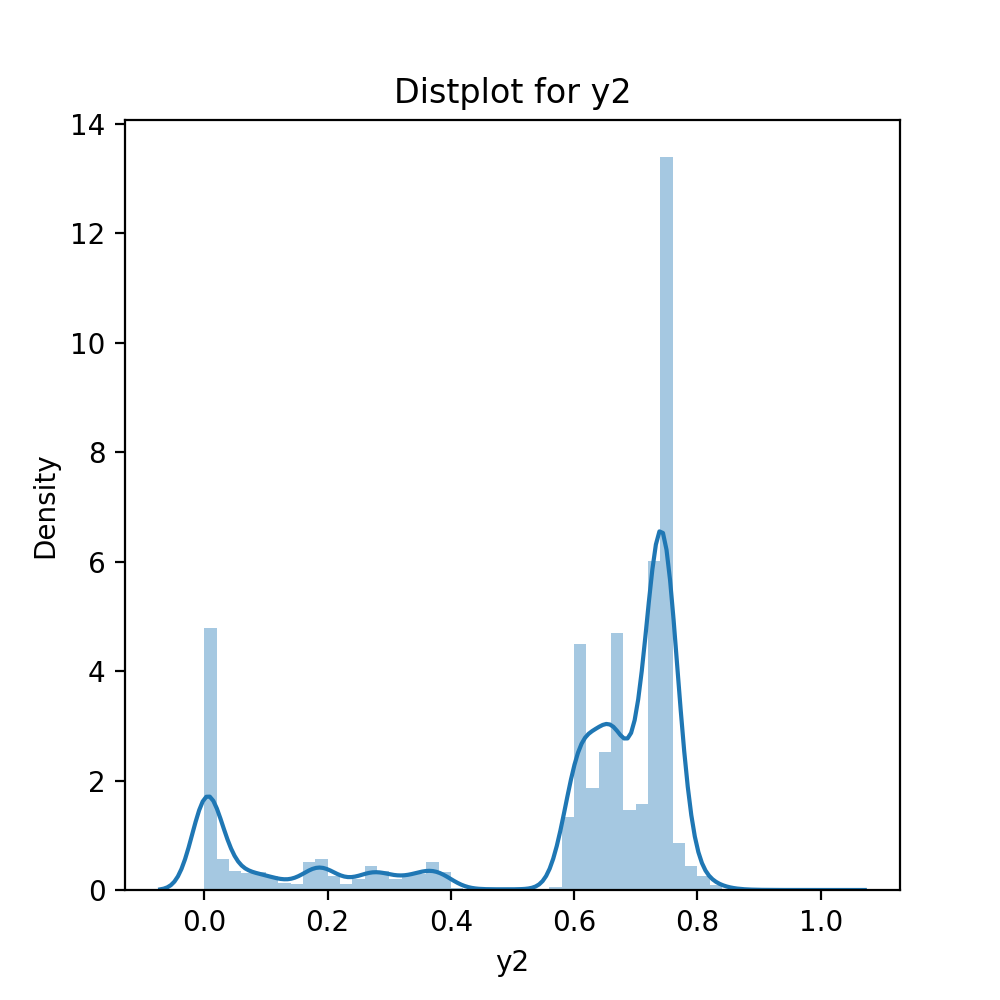
\includegraphics[width=1\linewidth]{y2postscaling}
        \caption{Distribuzione di y2 dopo il min-max-scaling.}
        \label{fig:distpostscaling:y2}
    \end{subfigure}
    \caption{Distribuzione di variabili dopo il min-max-scaling.}
    \label{fig:distpostscaling}
\end{figure}

In figura \ref{fig:distpostscaling} invece sono mostrati i grafici delle distribuzioni delle stesse variabili dopo aver subito la trasformazione del min-max-scaling, come si vede il valore è compreso tra 0 e 1 ma l'andamento è lo stesso e la distribuzione mantiene la stessa forma, a prova del fatto che i dati mantengono le stesse informazioni rappresentative. Grazie a quest'operazione di trasformazione delle features i modelli saranno più efficienti in fase di training e veloci.

\subsection{Decision Tree}

\subsection{Support Vector Machine}

\subsection{Reti neurali}

\subsection{Metriche di valutazione}
\section{Risultati e discussione}\label{sec:risultati}
In questa sezione verranno discussi e confrontati i risultati che i tre modelli nelle varie versioni hanno raggiunto nella fase di testing sul test set.

Dalla tabella \ref{tab:resdt} si nota che la versione migliore del Decision tree è la terza, quella in ensemble, infatti supera le prime due in tutte le metriche e raggiunge una precisione molto alta.

\begin{table}[h] 
\centering
\begin{tabular}{l l l l l}
\hline
\textbf{Versione} & \textbf{Accuracy bilanciata} & \textbf{Precision} & \textbf{Recall} & \textbf{F1-score}\\
\hline
Versione 1 & 0.976 & 0.986 & 0.986 & 0.986 \\
Versione 2 & 0.973 & 0.984 & 0.984 & 0.984 \\
\textbf{Versione 3} & \textbf{0.993} & \textbf{0.996} & \textbf{0.996} & \textbf{0.996} \\
\hline
\end{tabular}
\caption{Prestazioni delle varianti del Decision tree.}
\label{tab:resdt}
\end{table}

In tabella \ref{tab:ressvm} invece vediamo i risultati delle tre versioni del modello SVM, dai quali si deduce che anche in questo caso la versione migliore è quella in ensemble in quanto migliora di circa il 15-20\% i risultati delle prime due versioni, grazie proprio alla combinazione dei risultati di più modelli, cosiddetti weak learner, in un risultato unico. I risultati raggiunti comunque non sono soddisfacenti e non sono paragonabili a quelli che garantisce il Decision tree.

\begin{table}[h] 
\centering
\begin{tabular}{l l l l l}
\hline
\textbf{Versione} & \textbf{Accuracy bilanciata} & \textbf{Precision} & \textbf{Recall} & \textbf{F1-score}\\
\hline
Versione 1 & 0.420 & 0.551 & 0.490 & 0.482 \\
Versione 2 & 0.440 & 0.500 & 0.452 & 0.434 \\
\textbf{Versione 3} & \textbf{0.610} & \textbf{0.675} & \textbf{0.655 } & \textbf{0.620} \\
\hline
\end{tabular}
\caption{Prestazioni delle varianti dell'SVM.}
\label{tab:ressvm}
\end{table}

In tabella \ref{tab:resnn} sono confrontati i risultati della rete neurale nelle tre versioni, e come si vede la migliore è anche in questo caso la terza, anche se la differenza con la seconda versione è minima quindi l'incremento di prestazioni dato dall'ensemble è trascurabile in questo caso, seppur non nullo.

\begin{table}[h] 
\centering
\begin{tabular}{l l l l l}
\hline
\textbf{Versione} & \textbf{Accuracy bilanciata} & \textbf{Precision} & \textbf{Recall} & \textbf{F1-score}\\
\hline
Versione 1 & 0.963 & 0.981 & 0.981 & 0.981 \\
Versione 2 & 0.986 & 0.991 & 0.991 & 0.991 \\
\textbf{Versione 3} & \textbf{0.990} & \textbf{0.993} & \textbf{0.993} & \textbf{0.993} \\
\hline
\end{tabular}
\caption{Prestazioni delle varianti della rete neurale.}
\label{tab:resnn}
\end{table}

Infine in tabella \ref{tab:resbest} sono messi a confronto i tre modelli nelle loro versioni migliori, come si vede l'algoritmo che performa meglio è il Decision tree, anche se la rete neurale ha prestazioni molto simili, solo leggermente inferiori, invece la SVM ha prestazioni nettamente inferiori e quindi è sconsigliata in questo problema.

\begin{table}[h] 
\centering
\begin{tabular}{l l l l l}
\hline
\textbf{Modello} & \textbf{Accuracy bilanciata} & \textbf{Precision} & \textbf{Recall} & \textbf{F1-score}\\
\hline
\textbf{Decision Tree} & \textbf{0.993} & \textbf{0.996} & \textbf{0.996} & \textbf{0.996} \\
SVM & 0.610 & 0.675 & 0.655 & 0.620 \\
Rete neurale & 0.990 & 0.993 & 0.993 & 0.993 \\
\hline
\end{tabular}
\caption{Confronto tra le migliori versioni dei tre modelli analizzati.}
\label{tab:resbest}
\end{table}

In tutti e tre i modelli la versione migliore è risultata essere la terza, grazie all'incremento di prestazioni garantito dall'ensemble, nel caso però della SVM e della rete neurale questo avviene a un costo di efficienza in termini di velocità, infatti applicando il metodo Bagging il processo di training è rallentato considerevolmente rispetto alle prime due versioni. Questo rallentamento non avviene nel caso del Decision tree, infatti il RandomForest ha tempi paragonabili alla versione non in ensemble. 

In figura \ref{fig:conf} sono rappresentate le tre confusion matrix delle versioni migliori dei tre modelli, i valori sono normalizzati in questo caso, quindi non sono mostrati i valori assoluti ma la percentuale sul totale. Come si vede le matrici del Decision tree e della rete neurale hanno valori prossimi a uno sulla diagonale principale, il che significa che i valori predetti per una classe sono quasi tutti corretti. Al contrario la matrice del modello SVM ha valori minori nella diagonale principale, a dimostrazione del fatto che le prestazioni di questo algoritmo non sono eccellenti.  In particolare l'algoritmo ha pessime prestazioni con le classi \textit{3} e \textit{4}, mentre sulle classi \textit{0, 1 e 2} ha valori paragonabili a quelli ottenuti dal Decision tree e dalla rete neurale. 

\begin{figure}[h]
    \centering
    \begin{subfigure}[t]{0.4\textwidth}
        \centering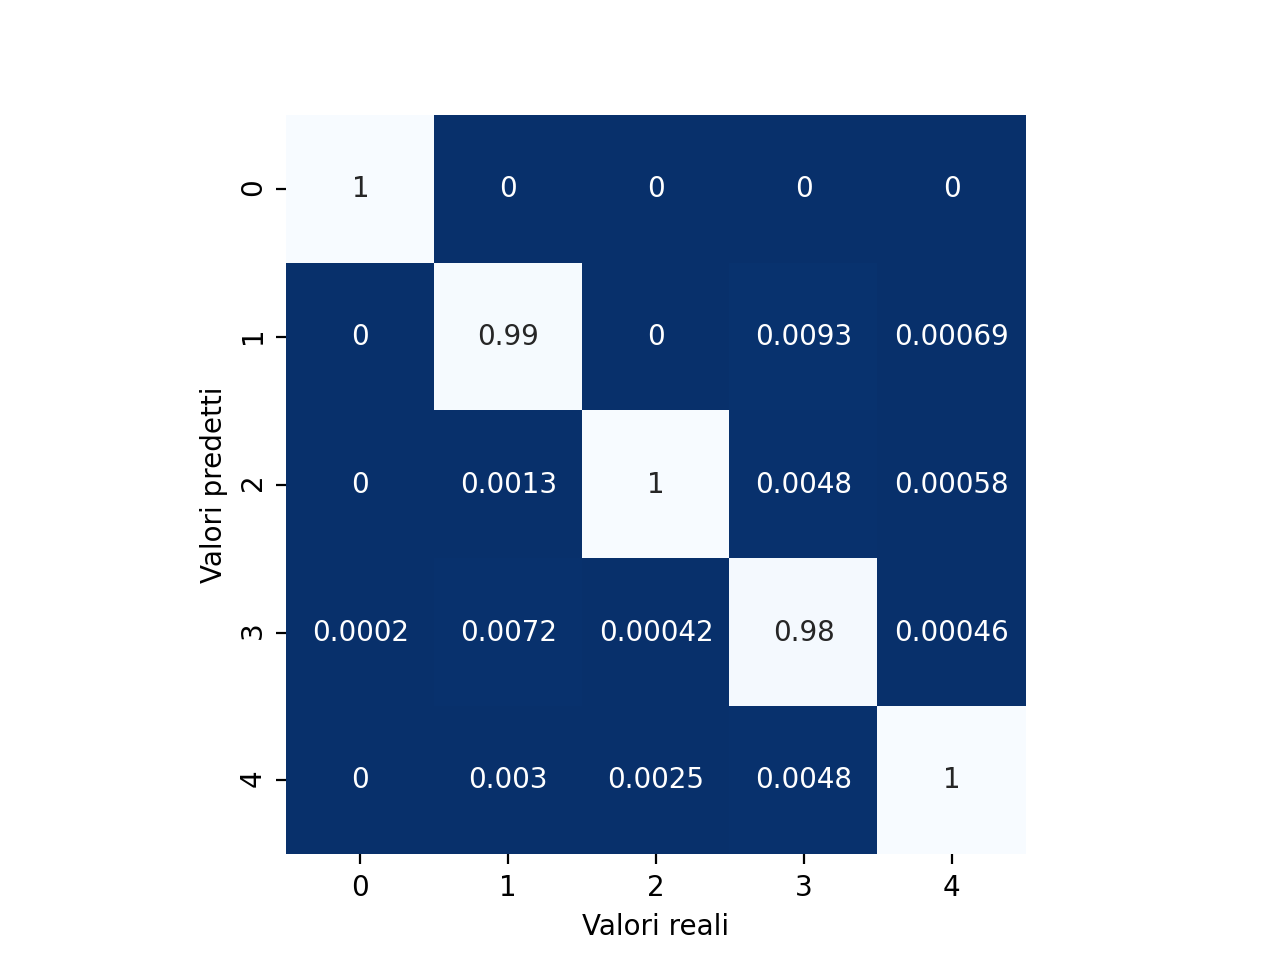
\includegraphics[width=1\linewidth]{confdt}
        \caption{Confusion matrix della terza versione del Decision tree.}
        \label{fig:conf:dt}
    \end{subfigure}
    %
    \begin{subfigure}[t]{0.4\textwidth}
        \centering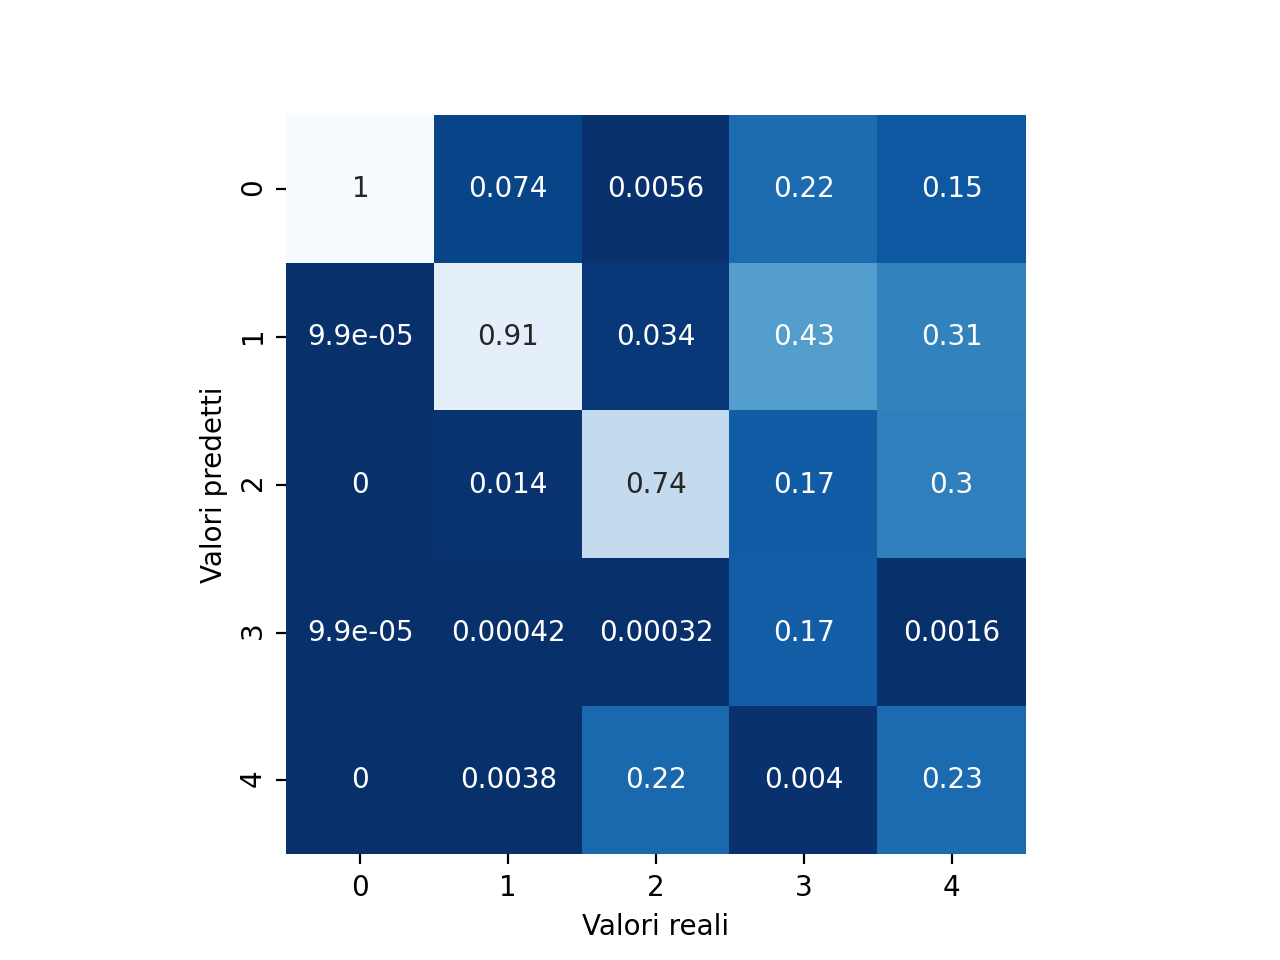
\includegraphics[width=1\linewidth]{confsvm}
        \caption{Confusion matrix della terza versione dell'SVM.}
        \label{fig:conf:svm}
    \end{subfigure}
    %
    \\
    \begin{subfigure}[t]{0.4\textwidth}
        \centering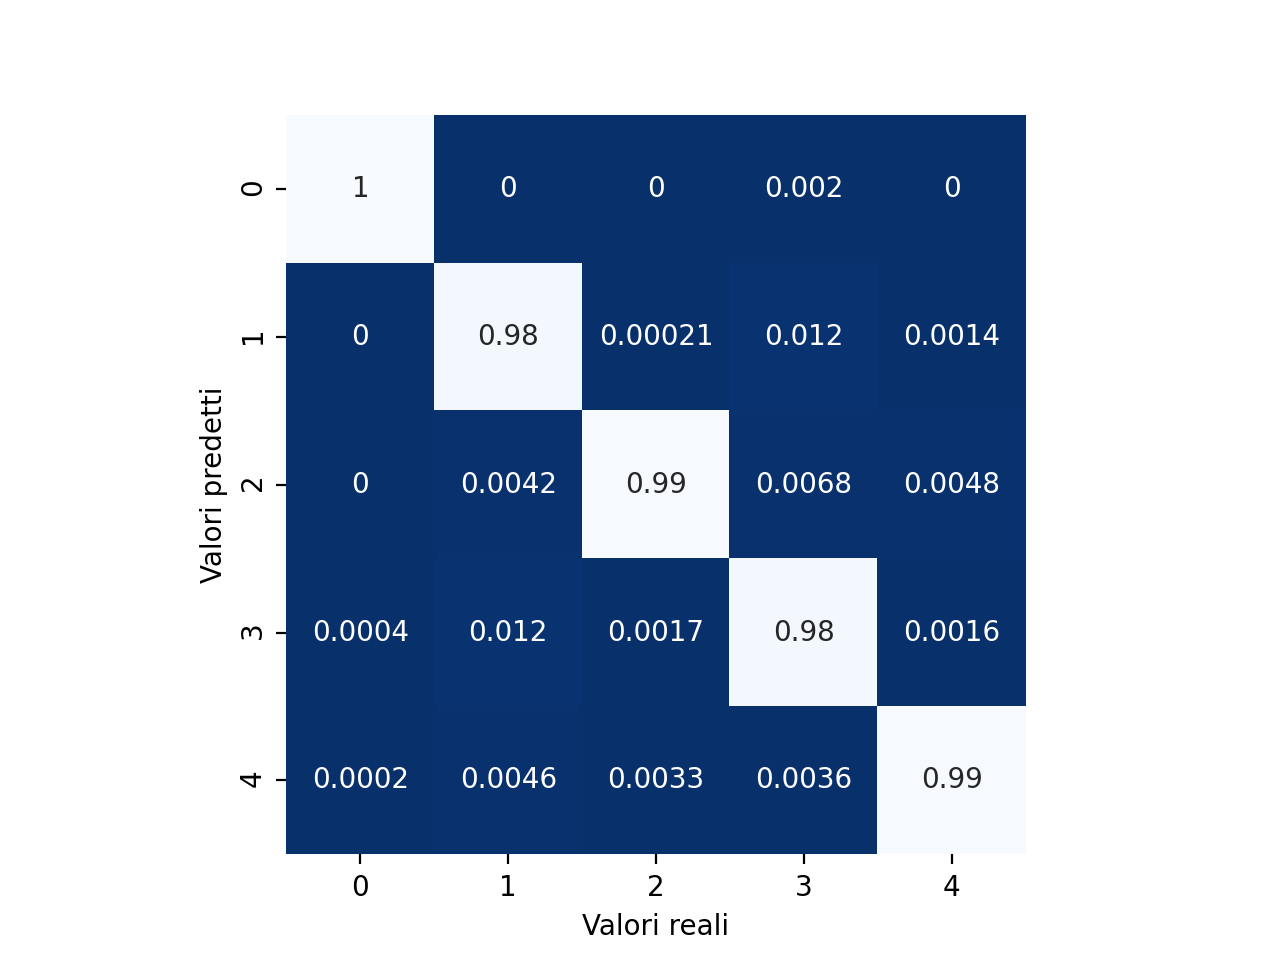
\includegraphics[width=1\linewidth]{confnn}
        \caption{Confusion matrix della terza versione della rete neurale.}
        \label{fig:conf:nn}
    \end{subfigure}
    %
    \caption{Confusion matrix dei tre modelli migliori.}
    \label{fig:conf}
\end{figure}

Per questo progetto sia la SVM che la rete neurale sono state testate con dei valori per gli iperparametri non ottimali, infatti per questioni di tempo e hardware a disposizione è stato deciso di non usare valori troppo alti per alcuni degli iperparametri, che probabilmente avrebbero portato a risultati migliori ma a discapito del tempo di training e di model selection, tenendo conto anche del fatto che il dataset usato contiene un notevole numero di sample, anche questo contribuisce ad allungare i tempi di addestramento. Nonostante ciò comunque la rete neurale è riuscita a performare molto bene avvicinandosi molto all'algoritmo che è risultato migliore, il Decision tree; la SVM invece non ha raggiunto questi risultati.

Per concludere, quindi, per tutti i modelli testati la versione migliore risulta essere la terza, cioè quella in ensemble, anche se per la rete neurale il miglioramento è molto piccolo e visto il peggioramento che il metodo di ensemble introduce in termini di velocità potrebbe essere conveniente utilizzare la versione numero due, in quanto ha tempi di addestramento minori e prestazioni molto simili. Tra i tre modelli infine il più prestante risulta essere il Decision tree in ensemble, quindi nello specifico il RandomForest, con gli iperparametri descritti nella tabella \ref{tab:dtv3}.
\section{\LaTeX{} Examples}
The following examples should help you to write your technical report using \LaTeX{}. You'll find here the examples of tables, figures, citations and references. For other features of \LaTeX{}, see tutorials on \href{https://www.overleaf.com/learn}{\textbf{Overleaf}} or use this \href{https://wch.github.io/latexsheet/}{\textbf{cheatsheet}}. To work with this template, download its entire folder (including /sections, /bibliography and /figures), and run your \LaTeX{} editor like \href{https://www.overleaf.com}{\textbf{Overleaf}}.


\subsection*{Example Citation}
Example of citation: \cite{Smith_2013} and \cite{Smith_2012}. 


\subsection*{Example References}
Example of table reference: see Table \ref{tab:example}. \\
Example of equation reference: see Equation \eqref{eq:emc}. \\
Example of reference to Section \ref{sec:sezione}. \\
Example of reference to Subsection \ref{ssec:sottosezione}. \\
Example of figure reference: see Figure \ref{fig:example}.\\
Example of subfigure reference: see Figure \ref{fig:multiple:example11}.\\


\subsection*{Example list}
\begin{itemize}
\item Bullet point one
\item Bullet point two
\item Nested list items:
\begin{itemize}
\item Nested item one
\item Nested item two
\end{itemize}
\end{itemize}

\subsection*{Enumerations}
\begin{enumerate}
\item Numbered list item one
\item Numbered list item two
\item Nested list items:
\begin{enumerate}
\item Nested item one
\item Nested item two
\end{enumerate}
\end{enumerate}


\subsection*{Example Table}

\begin{table}[h] 
\centering
\begin{tabular}{l l l}
\hline
\textbf{Treatments} & \textbf{Response 1} & \textbf{Response 2}\\
\hline
Treatment 1 & 0.0003262 & 0.562 \\
Treatment 2 & 0.0015681 & 0.910 \\
Treatment 3 & 0.0009271 & 0.296 \\
\hline
\end{tabular}
\caption{Table caption}
\label{tab:example}
\end{table}



\subsection*{Example Equation}
Equations within the text: $e = mc^2$. Equation with label on its own line:
\begin{equation} \label{eq:emc}
    e = mc^2
\end{equation}




\subsection*{Example Figures}

\begin{figure}[ht]
    \centering
\includegraphics[width=0.4\linewidth]{placeholder}
    \caption{An example of simple figure.}
    \label{fig:example}
\end{figure}

\begin{figure}[ht]
    \centering
    \begin{subfigure}[t]{0.4\textwidth}
        \centering
\includegraphics[width=1\linewidth]{placeholder}
        \caption{An example of multiple figures in one frame.}
        \label{fig:multiple:example11}
    \end{subfigure}
    %
    \begin{subfigure}[t]{0.4\textwidth}
        \centering
\includegraphics[width=1\linewidth]{placeholder}
        \caption{Next subfigure.}
        \label{fig:multiple:example12}
    \end{subfigure}
    %
    \\
    \begin{subfigure}[t]{0.4\textwidth}
        \centering
\includegraphics[width=1\linewidth]{placeholder}
        \caption{Subfigure on another line.}
        \label{fig:multiple:example21}
    \end{subfigure}
    %
    \begin{subfigure}[t]{0.4\textwidth}
        \centering
\includegraphics[width=1\linewidth]{placeholder}
        \caption{Yet another subfigure.}
        \label{fig:multiple:example22}
    \end{subfigure}
    \caption{More figures in appendix.}
    \label{fig:multiple}
\end{figure}

%----------------------------------------------------------------------------------------
%	Bibliography
%----------------------------------------------------------------------------------------
\bibliography{bibliography/sample}{}
\bibliographystyle{plain}

\end{document}